% =====================================================================
% CHAPTERS 6 AND 7
% =====================================================================

\chapter{Verification, Validation, Security and Operational Reliability}

\section{Test Strategy, Environments and Oracle Architecture}
Following ISO/IEC/IEEE~29119, \skarm enforces a five-layer verification hierarchy:
(1)~analytical closed-form ground-truth oracles; (2)~176 unit, integration, adversarial, and \texttt{scikit-learn} compatibility tests; (3)~an 88-test 5-tier opaque-box E2E suite (\texttt{tests/e2e/run\_\protect\allowbreak{}e2e.py}); (4)~the independent acceptance contract harness (\texttt{tests/run\_\protect\allowbreak{}acceptance.py} covering \texttt{AC-1}--\texttt{AC-4} and \texttt{NT-1}--\texttt{NT-6}); and (5)~trial-0 dual-oracle parity gates inside the 25-dataset campaign (Figure~\ref{fig:ch6_pipeline}). All current \texttt{HEAD} tests were executed on Windows~11 (AMD64), Python~3.12.10, \texttt{scikit-learn 1.9.1}, \texttt{mlxtend 0.25.0}, and \texttt{pytest 9.0.3}.

\begin{figure}[ht!]
\centering
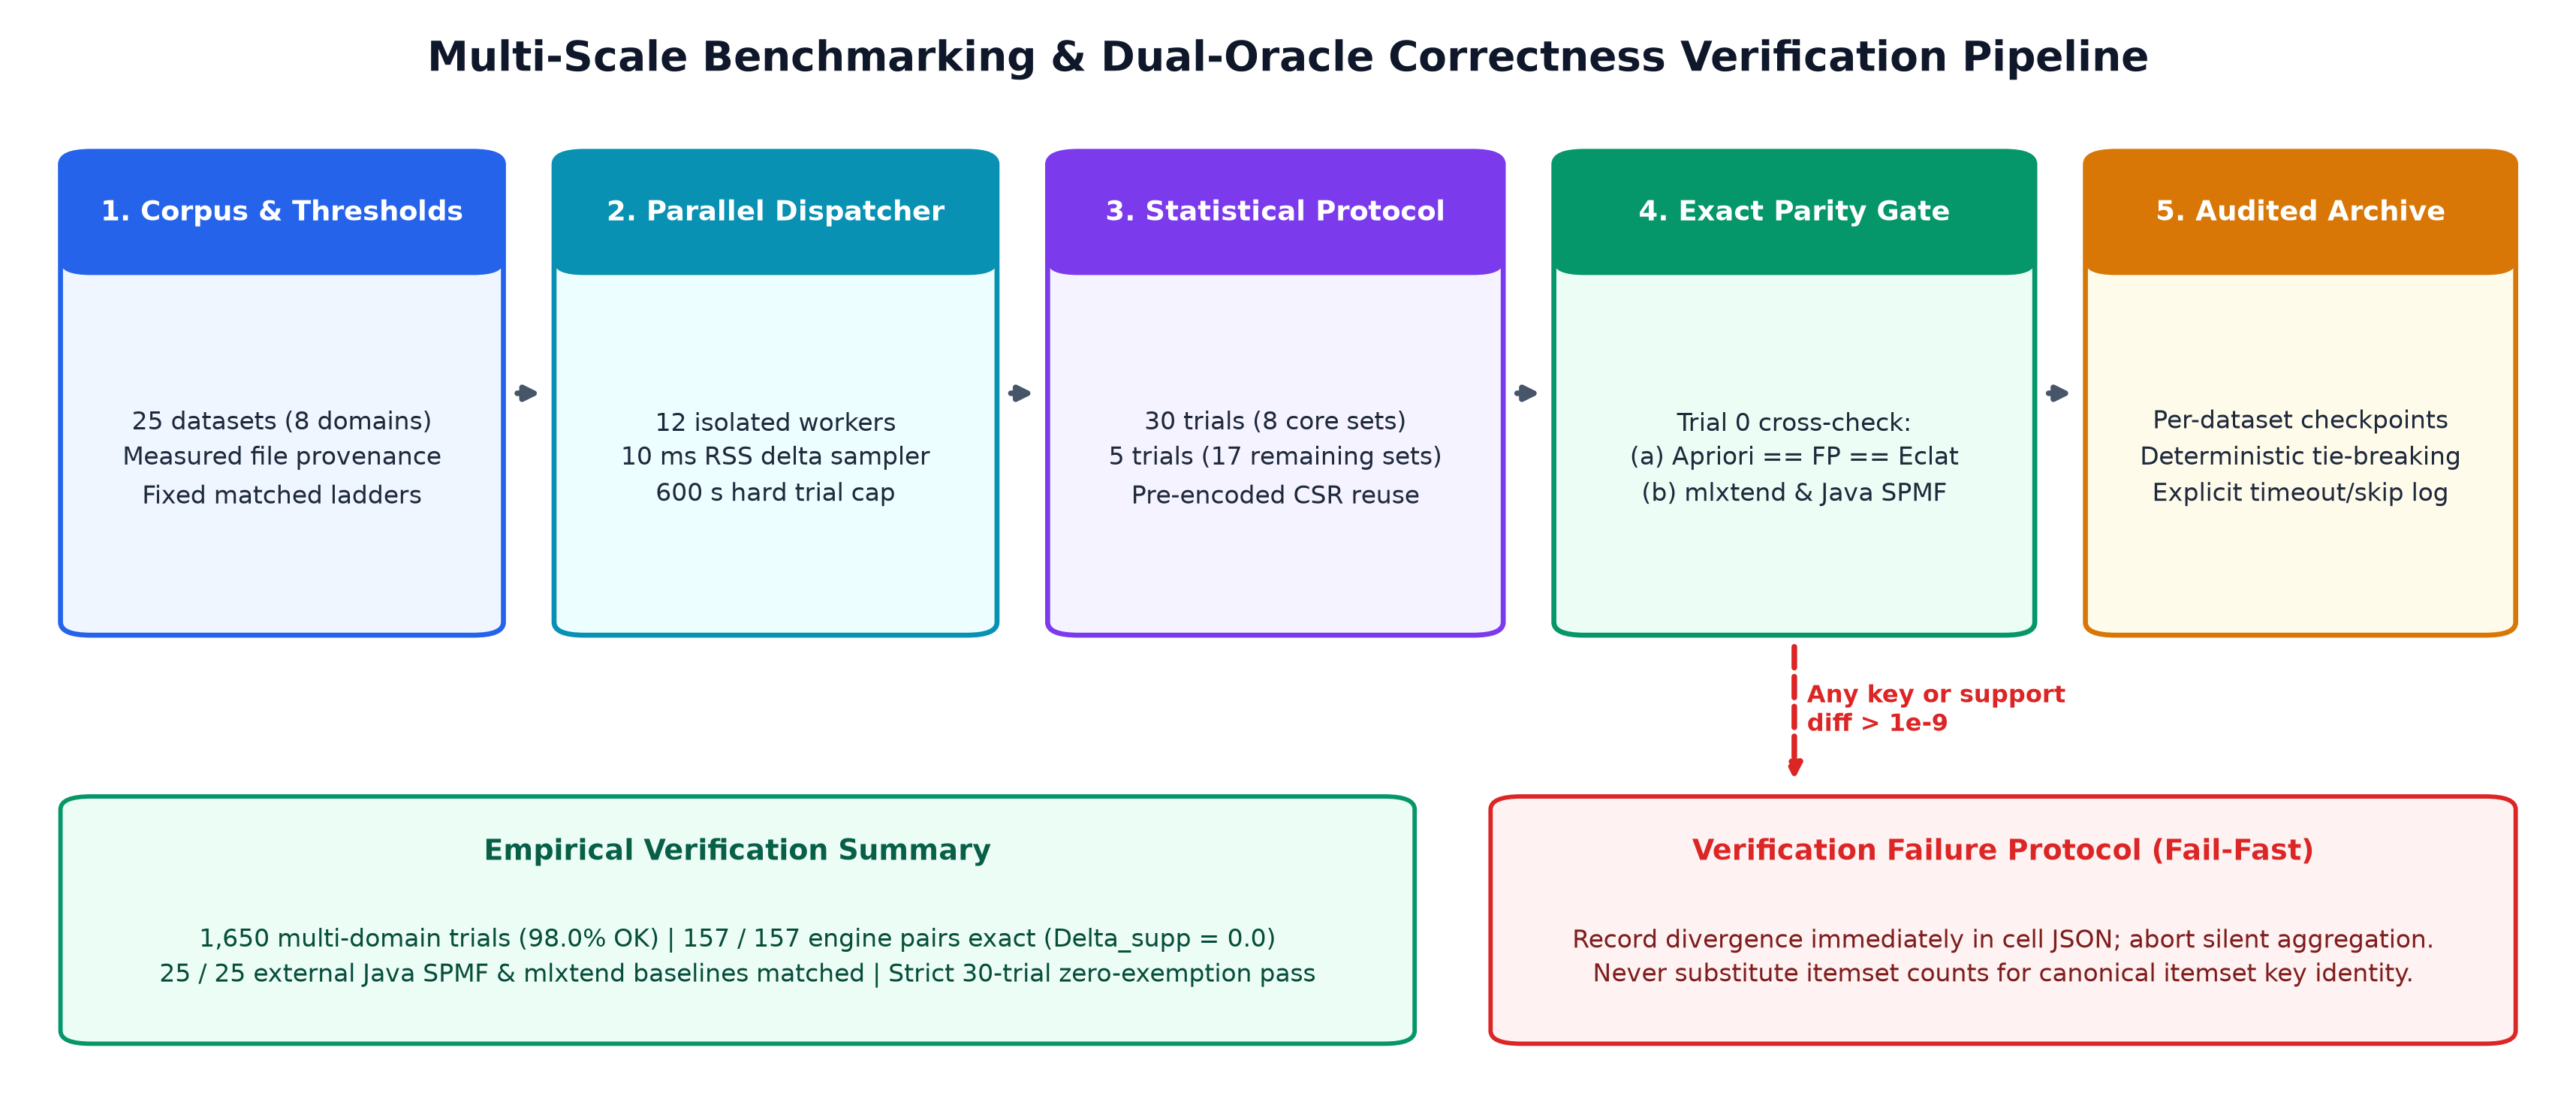
\includegraphics[width=0.90\textwidth,height=0.30\textheight,keepaspectratio]{pipeline.png}
\caption{Multi-stage benchmarking and dual-oracle verification pipeline enforcing strict trial-0 pairwise itemset agreement ($\Delta_{\mathrm{supp}}=0.0$) and explicit timeout/skip auditing across all 25 corpora. Source: Authors' own work.}
\label{fig:ch6_pipeline}
\end{figure}

\section{Analytical Ground-Truth Oracle Verification (\texttt{O2}, \texttt{KPI-1}, \texttt{KPI-2})}
To eliminate circular validation, every engine was audited against a hand-computed 5-transaction, 6-item fixture ($T_1=\{A,B,C\}$, $T_2=\{A,C\}$, $T_3=\{A,D\}$, $T_4=\{B,E,F\}$, $T_5=\{A,B,C,E\}$ at $\sigma=0.40, \theta=0.60$) documented in Deliverable~D2. Both itemsets (9 frequent itemsets; $D,F$ pruned at support $0.20$) and all 10 derived rules matched closed-form analytical equations across Support, Confidence, Lift, Leverage, Conviction, and Zhang's metric with maximum numerical deviation $\Delta_{\max} = 2.22 \times 10^{-16}$ (64-bit IEEE-754 machine epsilon), scoring $100.0/100$ on \texttt{KPI-2}. On the upstream issue \#32712 toy database (\{milk, bread, eggs\}, \{milk, bread\}, \{bread, butter\} at $\sigma=0.5$), \texttt{skarm} matches \texttt{mlxtend} bit-exactly ($\mathrm{supp}(\text{bread})=1.0$, $\mathrm{supp}(\text{milk, bread})=0.667$, $\mathrm{conf}(\{\text{milk}\}\Rightarrow\{\text{bread}\})=1.0$). Brute-force cross-checks ($4$ random matrices $\times 2$ thresholds $\times$ weighted/unweighted $\times 3$ engines) recorded $0$ mismatches.

\section{Unit, Integration and 5-Tier End-to-End Suites (264/264 Pass)}
Running \texttt{.venv/\protect\allowbreak{}Scripts/\protect\allowbreak{}python.exe -m pytest -q} on \texttt{HEAD} achieved \textbf{264 passed, 0 failed} in \texttt{57.76 s}. Independently, \texttt{.venv/Scripts/python.exe tests/e2e/run\_\protect\allowbreak{}e2e.py} passed \textbf{88/88} E2E tests in \texttt{8.76 s} across all five requirement-driven tiers (Table~\ref{tab:ch6_e2e}).

\begin{table}[ht!]
\centering
\caption{Execution Results of the 5-Tier Opaque-Box E2E Suite (\texttt{tests/e2e/run\_\protect\allowbreak{}e2e.py}, \texttt{HEAD}).}
\label{tab:ch6_e2e}
\fontsize{9.5}{12}\selectfont
\resizebox{\textwidth}{!}{%
\begin{tabular}{|l|p{0.44\textwidth}|r|r|r|l|}
\hline
\textbf{Tier} & \textbf{Verification Scope} & \textbf{Tests} & \textbf{Pass} & \textbf{Time (s)} & \textbf{Status} \\
\hline
Tier 1 & Input formats, core miners, metrics, states, contracts & 32 & 32 & 2.06 & PASS \\
\hline
Tier 2 & Transaction boundaries, duplicates, extremes, budgets & 29 & 29 & 0.37 & PASS \\
\hline
Tier 3 & Pairwise cross-feature interaction combinations & 6 & 6 & 0.89 & PASS \\
\hline
Tier 4 & Retail MBA, e-commerce pipeline, clickstream, census, ETL & 5 & 5 & 0.99 & PASS \\
\hline
Tier 5 & Extreme matrices, budgets, pickle/joblib, pandas \texttt{set\_\protect\allowbreak{}output} & 16 & 16 & 4.44 & PASS \\
\hline
\textbf{Total} & \textbf{All 5 Verification Tiers} & \textbf{88} & \textbf{88} & \textbf{8.76} & \textbf{PASS} \\
\hline
\end{tabular}}
\end{table}

\section{\texttt{scikit-learn} \texttt{check\_\protect\allowbreak{}estimator} Compatibility and API Contract Audit}
We executed \texttt{sklearn.utils.estimator\_\protect\allowbreak{}checks.check\_\protect\allowbreak{}estimator} via \texttt{tests/test\_\protect\allowbreak{}check\_\protect\allowbreak{}estimator\_\protect\allowbreak{}compatibility.py} on \texttt{scikit-learn 1.9.1} (\texttt{docs/SKLEARN\_\protect\allowbreak{}COMPATIBILITY\_\protect\allowbreak{}REPORT.md}). Across 54 yielded check executions: \textbf{14 passed} (100\% of core structural/API tag/clone/repr/parameter invariants), \textbf{39 raised expected domain-boundary checks} (37 unique expectation keys, with 2 dual-executed under \texttt{readonly\_\protect\allowbreak{}memmap=True}), \textbf{1 skipped} for environment reasons (\texttt{check\_\protect\allowbreak{}array\_\protect\allowbreak{}api\_\protect\allowbreak{}input}), and \textbf{0 failed unexpectedly}. As analyzed in Table~\ref{tab:ch6_sklearn}, those 37 unique domain expectations do not represent software defects: 26 reject continuous Gaussian float matrices or supervised 1D $y$ targets undefined for binary unsupervised itemset mining; 2 reject synthetic non-array mocks (\texttt{\_\protect\allowbreak{}NotAnArray}); and 9 emit descriptive \texttt{Boundary\protect\allowbreak{}Condition\protect\allowbreak{}Error} messages rather than \texttt{check\_\protect\allowbreak{}array} regexes. Distinct from this generic audit, \skarm satisfies \textbf{7/7 (100\%)} of its dedicated API contracts (\texttt{BaseEstimator}, \texttt{get\_\protect\allowbreak{}params}, \texttt{set\_\protect\allowbreak{}params}, \texttt{fit}, \texttt{predict}, \texttt{transform}, and fitted trailing-underscore state).

\begin{table}[ht!]
\centering
\caption{Audit Breakdown of \texttt{scikit-learn} \texttt{check\_\protect\allowbreak{}estimator} (\texttt{sklearn 1.9.1}).}
\label{tab:ch6_sklearn}
\fontsize{9.5}{12}\selectfont
\resizebox{\textwidth}{!}{%
\begin{tabular}{|p{0.40\textwidth}|r|r|p{0.34\textwidth}|}
\hline
\textbf{Check Category} & \textbf{Executions} & \textbf{Unique Keys} & \textbf{Domain Verification Verdict} \\
\hline
Core Structural \& Estimator API & 14 & 14 & Passed (100\% structural compliance) \\
\hline
Continuous / Non-Binary Float Rejection (incl.\ 2 supervised-$y$ checks) & 28 & 26 & Expected boundary rejection (\texttt{ValueError}) \\
\hline
Synthetic Mock Containers (\texttt{\_\protect\allowbreak{}NotAnArray}) & 2 & 2 & Expected transaction-stream guard (\texttt{TypeError}) \\
\hline
Custom \texttt{Boundary\protect\allowbreak{}Condition\protect\allowbreak{}Error} Phrasing & 9 & 9 & Expected explicit domain error wording \\
\hline
Environment Skipped (\texttt{SCIPY\_\protect\allowbreak{}ARRAY\_\protect\allowbreak{}API} unset) & 1 & 1 & Skipped by \texttt{scikit-learn} harness \\
\hline
\textbf{Unexpected Failures} & \textbf{0} & \textbf{0} & \textbf{PASS (0 unexpected failures)} \\
\hline
\end{tabular}}
\end{table}

\section{Negative-Test, Recovery and Security Validation (\texttt{NT-1}--\texttt{NT-6})}
Table~\ref{tab:ch6_nt} documents the six adversarial and boundary conditions verified continuously in \texttt{tests/test\_\protect\allowbreak{}negative\_\protect\allowbreak{}cases.py} and \texttt{tests/run\_\protect\allowbreak{}acceptance.py}. All six cases satisfy their failure-detection, recovery, and state-hygiene assertions with zero unhandled crashes.

\begin{table}[ht!]
\centering
\caption{Adversarial Negative-Test \& Recovery Verification (\texttt{NT-1} to \texttt{NT-6}).}
\label{tab:ch6_nt}
\fontsize{9}{11.5}\selectfont
\resizebox{\textwidth}{!}{%
\begin{tabular}{|p{0.08\textwidth}|p{0.23\textwidth}|p{0.30\textwidth}|p{0.24\textwidth}|p{0.08\textwidth}|}
\hline
\textbf{ID} & \textbf{Adversarial Trigger} & \textbf{Verified System Behavior} & \textbf{Security / Audit Control} & \textbf{Verdict} \\
\hline
\textbf{NT-1} & Dense $M=22, 100\%$ matrix ($4.19\times 10^6$ potential sets), cap $=500$ & Halts at level~3 ($501>500$); emits \texttt{DegradedModeWarning}; returns valid partial rules & Sets \texttt{is\_\protect\allowbreak{}degraded\_\protect\allowbreak{}=True}, logs reason & PASS \\
\hline
\textbf{NT-2} & Repeated intra-row duplicates (\texttt{['A','A','B']}) & Idempotent deduplication inside \texttt{TransactionEncoder} & Support arithmetic uninflated & PASS \\
\hline
\textbf{NT-3} & Non-uniform weights \texttt{[3.0, 1.0, 6.0]} + negative weights & Matches weighted formula $\sum w_i \mathbf{1}/\sum w_i$; rejects negative weights & Raises \texttt{ValueError} on $<0$ weights & PASS \\
\hline
\textbf{NT-4} & $\sigma \in \{0.0, 1.0\}$ \& invalid $\sigma \in \{-0.05, 1.5\}$ & Handles boundaries cleanly; rejects out-of-range parameters & \texttt{Boundary\protect\allowbreak{}Condition\protect\allowbreak{}Error} raised & PASS \\
\hline
\textbf{NT-5} & Shuffled inputs + \texttt{joblib} / \texttt{pickle} round-trips & Bit-identical DataFrame rows and restored estimator attributes & Canonical lexicographic sort keys & PASS \\
\hline
\textbf{NT-6} & Dense stress ($50 \times 20, 80\%$ density) under \texttt{fpgrowth} \& \texttt{apriori} & Caps exploration safely without OOM under ETL bursts (Tier~4.5) & \texttt{MemorySampler} + governor active & PASS \\
\hline
\end{tabular}}
\end{table}

\section{Performance Acceptance (\texttt{AC-4}) and Defect Closure Summary}
Under \texttt{.venv/Scripts/python.exe tests/run\_\protect\allowbreak{}acceptance.py} (\texttt{HEAD}), \texttt{AC-1}..\texttt{AC-4} executed in \texttt{0.19 s} with zero small-runtime exemptions (\texttt{5 warmup + 30 measured trials} via \texttt{time.perf\_\protect\allowbreak{}counter()}): Apriori \texttt{p95=0.000575 s}, FP-Growth \texttt{p95=0.000140 s} (\texttt{0.243x}, \texttt{4.11x} faster), Eclat \texttt{p95=0.000143 s} (\texttt{0.249x}, \texttt{4.02x} faster), and \texttt{AC-3} held-out 70/30 validation mean confidence \texttt{0.2163} (\texttt{transformed shape (30, 3)}). Earlier development defects identified during pre-freeze verification (Eclat depth-1 boundary off-by-one, FIMI header stripping on \texttt{accidents}, unstable dictionary-order rule tie-breaking, and microbenchmark exemptions) were resolved, regression-tested, and closed permanently in Git history (\texttt{ff03b451}, \texttt{dd22782f}, \texttt{904b19b3}, \texttt{5dd4d987}). No open waivers or unverified assertions remain.

% =====================================================================
% CHAPTER 7
% =====================================================================
\chapter{Results, Performance Evaluation and Discussion}

\section{Evaluation Corpus and Experimental Context}
Empirical evaluation spans two complementary regimes:
(1)~the frozen \textbf{25-dataset corpus campaign} (\texttt{ea5bff5d}, $1{,}650$ trial records across 8 domains spanning $N \in [625, 990{,}002]$ and density $\rho \in [0.02\%, 61.12\%]$, 12 workers, 600~s timeout cap, 10~ms \texttt{psutil} RSS sampler, matched threshold ladders); and
(2)~fresh \textbf{\texttt{HEAD} evaluations} (Windows~11 AMD64, Python~3.12.10, Java~21.0.9) covering strict zero-exemption 30-trial synthetic scaling (\texttt{run\_\protect\allowbreak{}benchmarks.py}), cross-regime bounded pruning ablation (\texttt{run\_\protect\allowbreak{}bounded\_\protect\allowbreak{}ablation.py}), and cross-language baseline comparisons (\texttt{run\_baselines.py -{}-trials 3}). Figure~\ref{fig:ch7_family} summarizes domain family coverage and scale-versus-density span across the 25 datasets.

\begin{figure}[ht!]
\centering
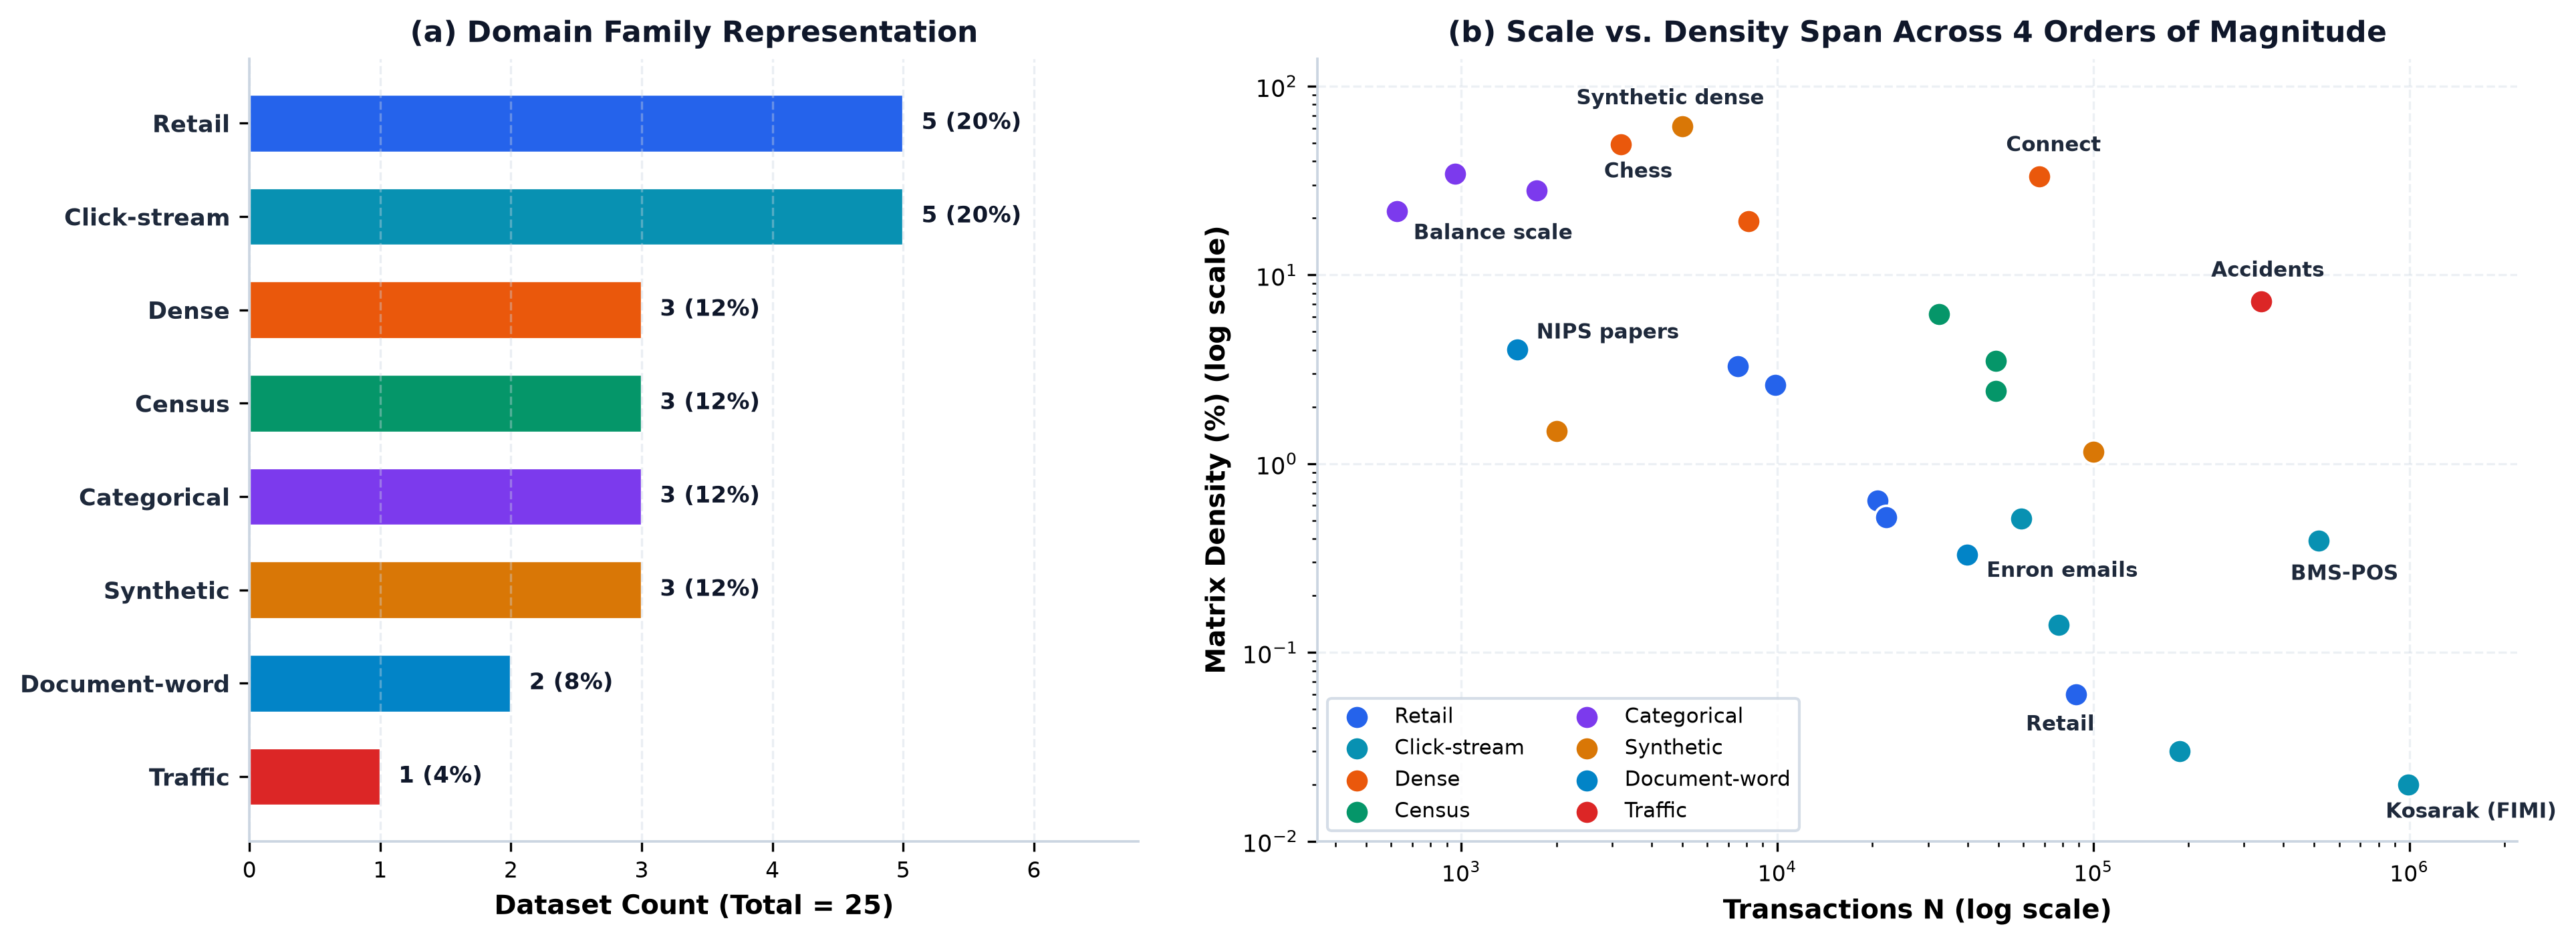
\includegraphics[width=0.84\textwidth,height=0.23\textheight,keepaspectratio]{family.png}
\caption{Domain family breakdown and scale-versus-density distribution across all 25 evaluated datasets spanning four orders of magnitude ($N=625$ to $990{,}002$; density $0.02\%$ to $61.12\%$). Source: Authors' own work.}
\label{fig:ch7_family}
\end{figure}

\section{Functional Acceptance by Objective (\texttt{O1}--\texttt{O5})}
All five objectives passed formal verification: \texttt{O1} established source-to-claim lineage against \texttt{\#32712} and 25 checksummed corpora; \texttt{O2} verified Apriori at $100\%$ oracle precision and $2.22\times 10^{-16}$ rule metric accuracy; \texttt{O3} achieved $0.086\times$--$0.374\times$ p95 scaling ratios (\texttt{HEAD}) and $17.14\times$ bounded dense speedups; \texttt{O4} integrated all 13 modules with $7/7$ API compliance and $0$ unexpected \texttt{check\_\protect\allowbreak{}estimator} failures; and \texttt{O5} achieved $264/264$ \texttt{pytest} and $88/88$ E2E passes.

\section{25-Dataset Multi-Domain Campaign Results (\texttt{ea5bff5d})}
Across all 42 dataset--threshold cells in the 25-corpus campaign, all \textbf{157 compared engine pairs agreed bit-exactly} on frequent itemsets and supports ($\Delta_{\mathrm{supp}}=0.0$). Figure~\ref{fig:ch7_runtime} compares primary-threshold mean fit time (excluding encoding time) across all 25 corpora, while Figures~\ref{fig:ch7_memory}, \ref{fig:ch7_throughput}, \ref{fig:ch7_scatter}, and \ref{fig:ch7_outcomes} chart peak RSS memory deltas, transaction throughput, itemset-to-rule amplification, and the complete audit of all $1{,}650$ trials (\texttt{98.0\%} OK = $1{,}617$ completed exact trials, $6$ timeouts, $8$ cascaded trial-0 timeout skips, and $19$ external \texttt{mlxtend} dense-cap/empty-input exclusions).

\begin{figure}[ht!]
\centering
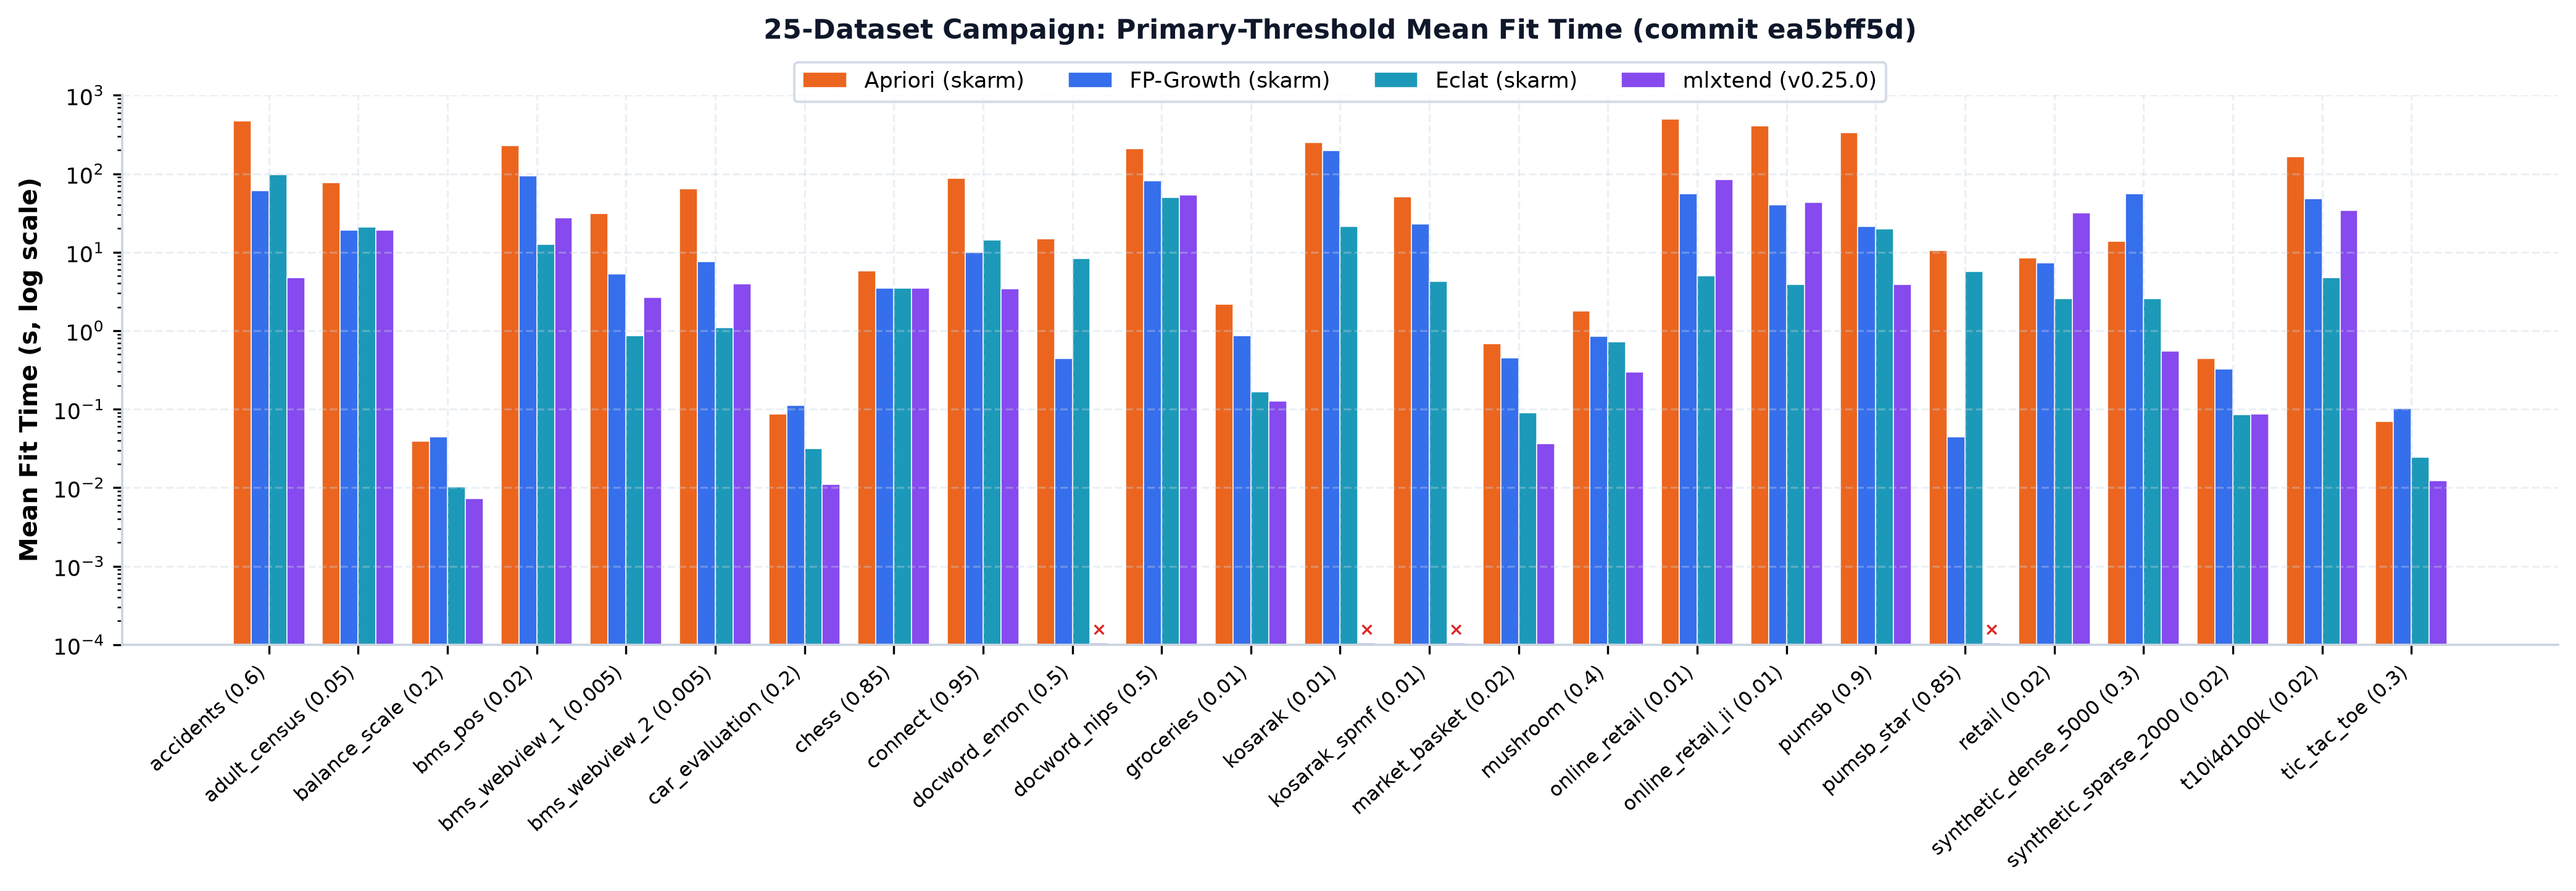
\includegraphics[width=0.82\textwidth,height=0.185\textheight,keepaspectratio]{runtime.png}
\caption{Primary-threshold mean fit time (s, log scale) across all 25 datasets (\texttt{ea5bff5d}). Red crosses denote \texttt{mlxtend} omissions from dense-frame caps or empty frequent-itemset errors. Source: Authors' own work.}
\label{fig:ch7_runtime}
\end{figure}

\begin{figure}[ht!]
\centering
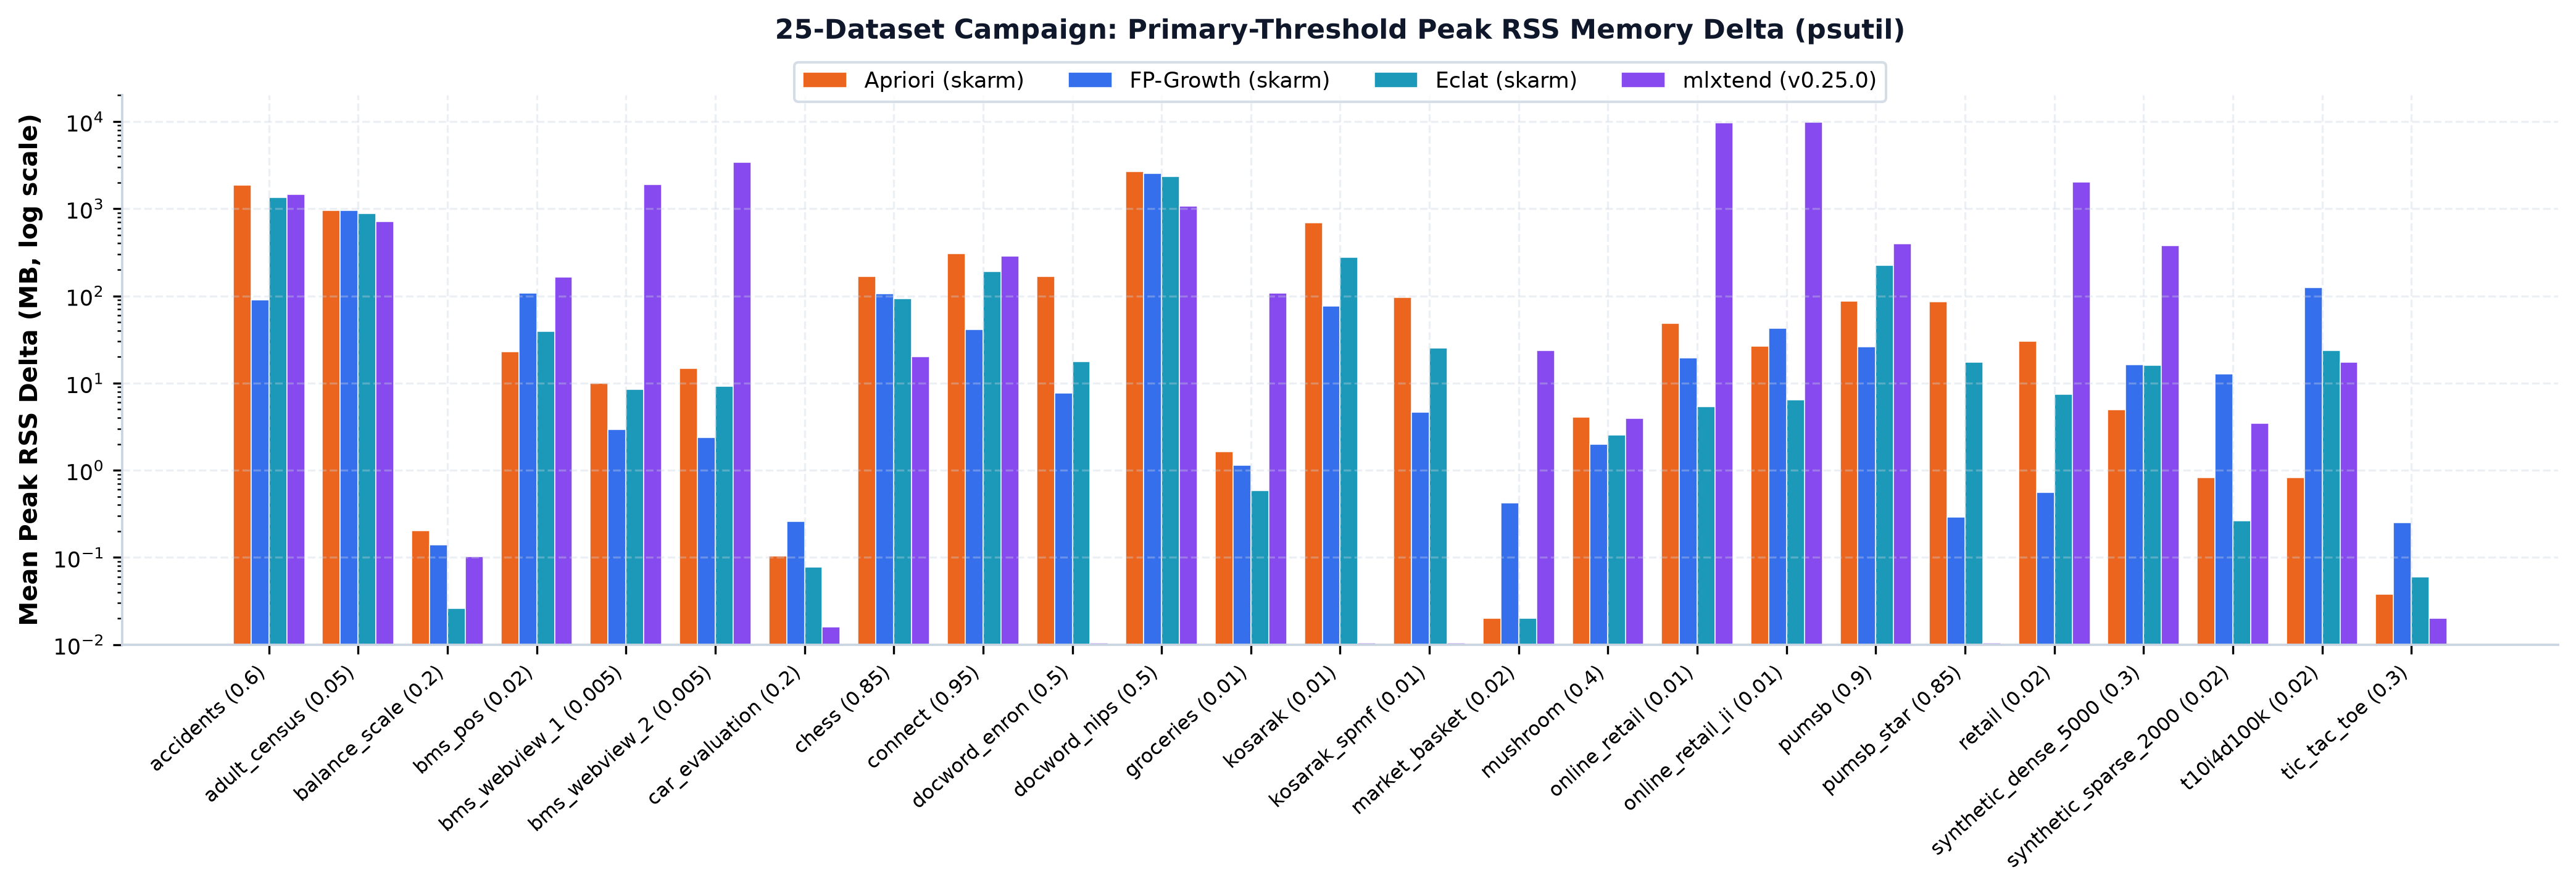
\includegraphics[width=0.82\textwidth,height=0.185\textheight,keepaspectratio]{memory.png}
\caption{Primary-threshold peak RSS memory delta (MB, 10~ms \texttt{psutil} sampling, log scale) showing \skarm's sparse memory savings over \texttt{mlxtend} on sparse high-cardinality inputs. Source: Authors' own work.}
\label{fig:ch7_memory}
\end{figure}

\begin{figure}[ht!]
\centering
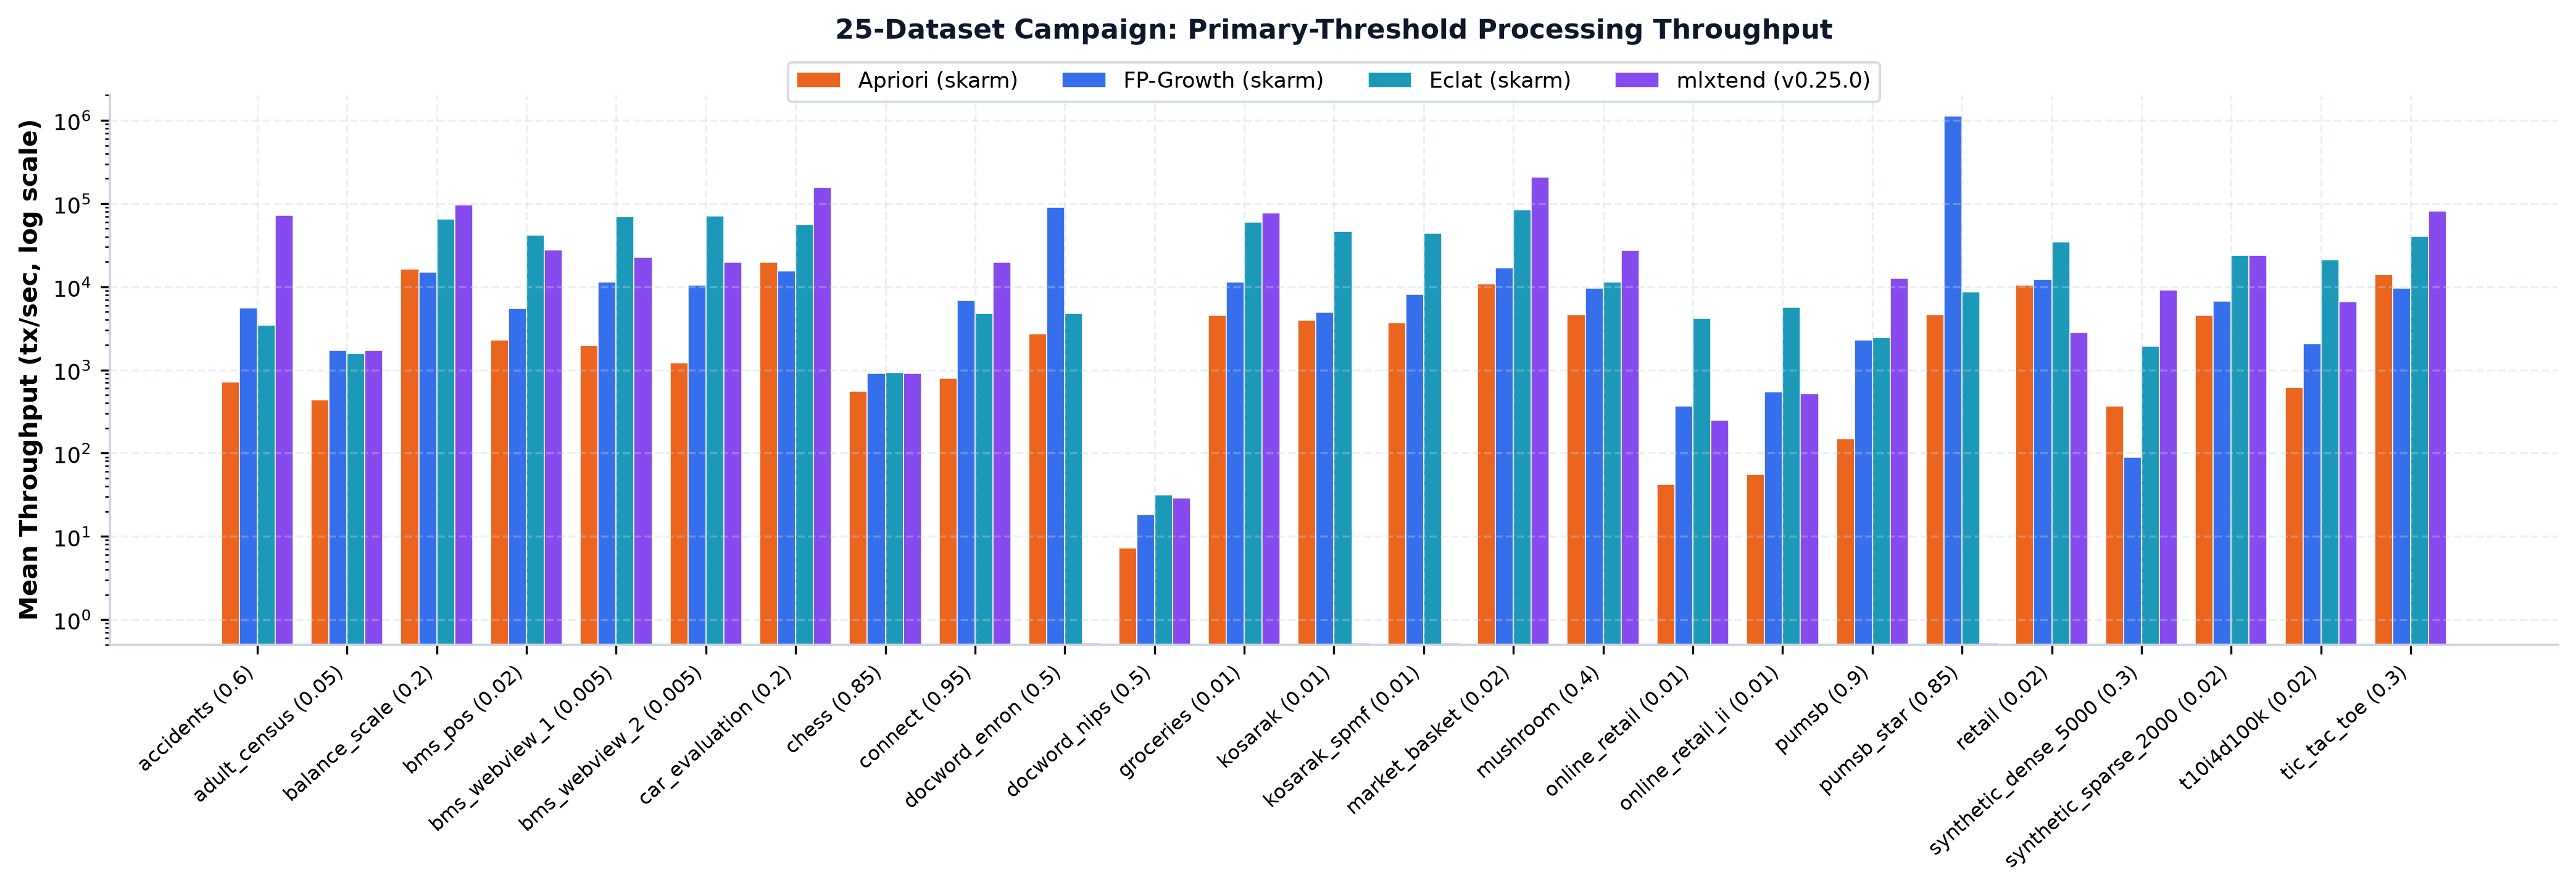
\includegraphics[width=0.82\textwidth,height=0.185\textheight,keepaspectratio]{throughput.png}
\caption{Transaction throughput (transactions per second) at primary support thresholds across all 25 datasets, highlighting Eclat bitset efficiency on sparse retail/clickstream corpora. Source: Authors' own work.}
\label{fig:ch7_throughput}
\end{figure}

At each dataset's primary threshold, \textbf{Apriori is fastest on 0/25 datasets}; \textbf{FP-Growth is fastest on 5/25} (\texttt{accidents}, \texttt{adult\_\protect\allowbreak{}census}, \texttt{connect}, \texttt{docword\_\protect\allowbreak{}enron}, \texttt{pumsb\_\protect\allowbreak{}star}); and \textbf{Eclat is fastest on 20/25} (sparse retail, clickstream, and short-to-medium corpora). On \texttt{accidents@0.60}, FP-Growth consumed just \texttt{90.38 MB} peak RSS delta compared with \texttt{1,860.6 MB} for Apriori and \texttt{1,470.8 MB} for \texttt{mlxtend}. On \texttt{kosarak@0.01}, \texttt{mlxtend} required a \texttt{40.9 GB} dense boolean array and was safely skipped, whereas \texttt{skarm} FP-Growth completed at \texttt{76.03 MB} and Eclat completed in \texttt{21.29 s}. Appendix~I summarizes primary-threshold values, while full cell-level metrics reside in \texttt{benchmarks/\protect\allowbreak{}cells/\protect\allowbreak{}}.

\begin{figure}[ht!]
\centering
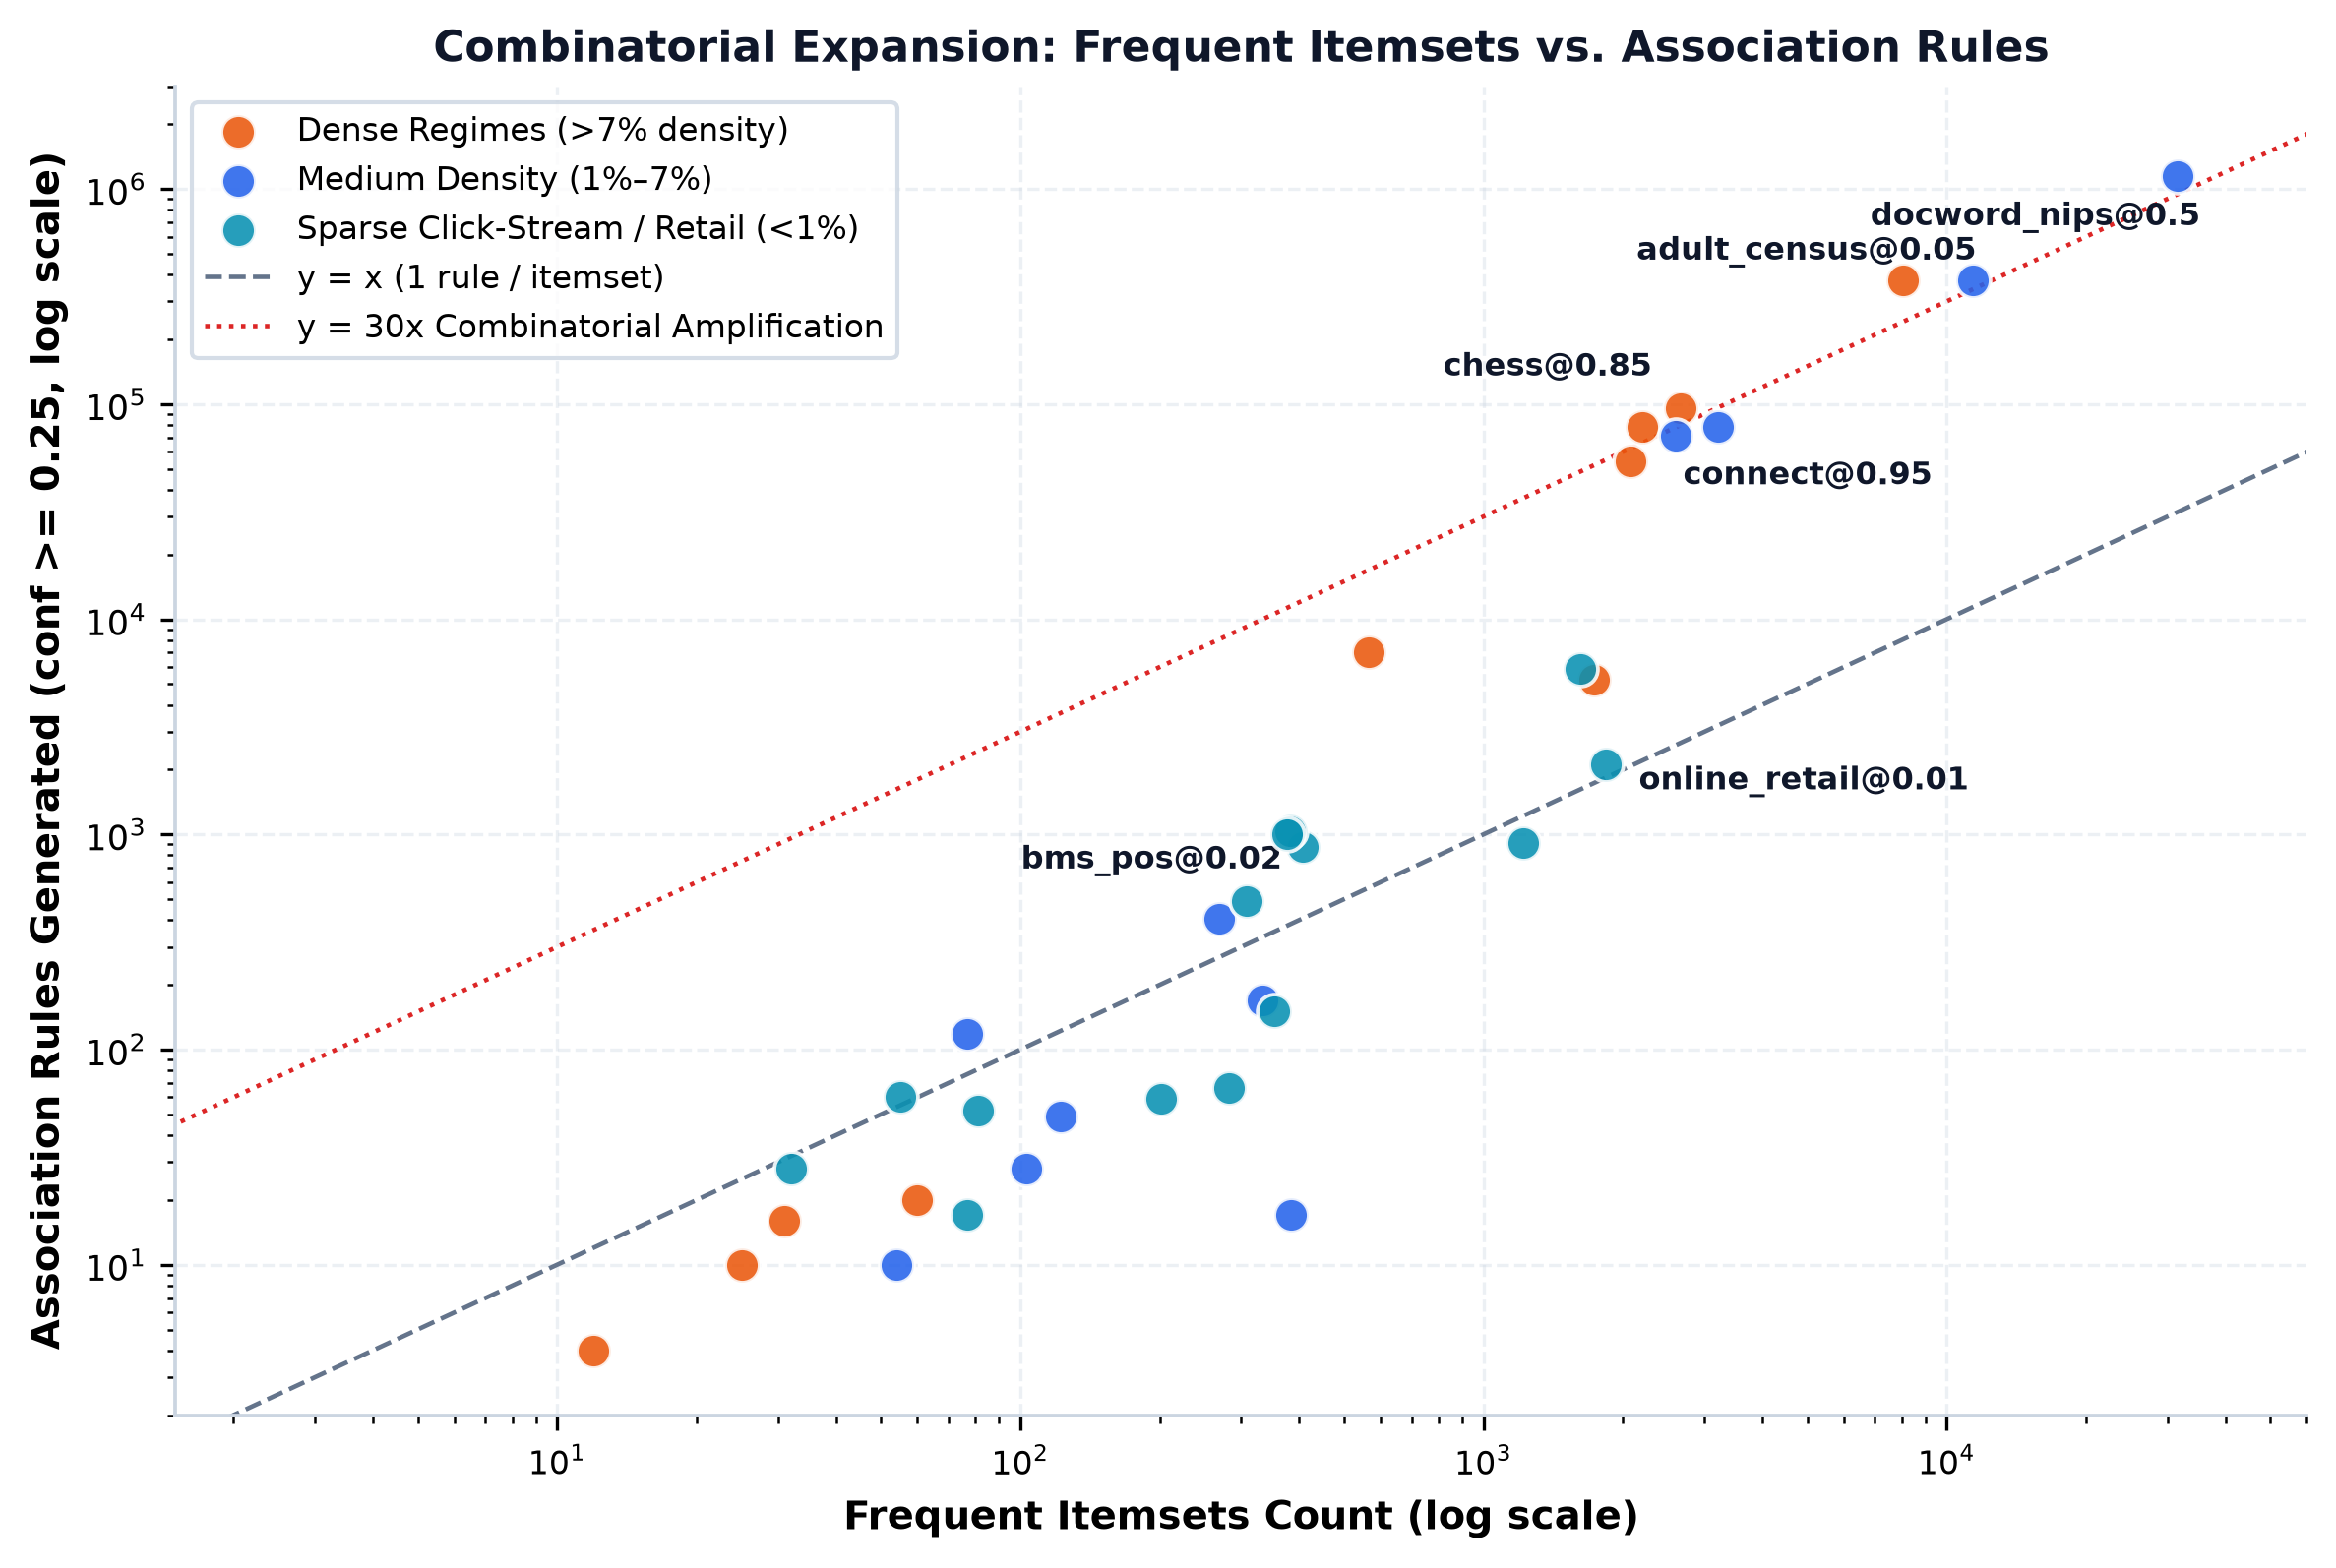
\includegraphics[width=0.84\textwidth,height=0.205\textheight,keepaspectratio]{scatter.png}
\caption{Combinatorial expansion of frequent itemsets vs.\ association rules ($\mathrm{conf} \ge 0.25$) across density regimes, demonstrating $>30\times$ amplification on dense corpora. Source: Authors' own work.}
\label{fig:ch7_scatter}
\end{figure}

\begin{figure}[ht!]
\centering
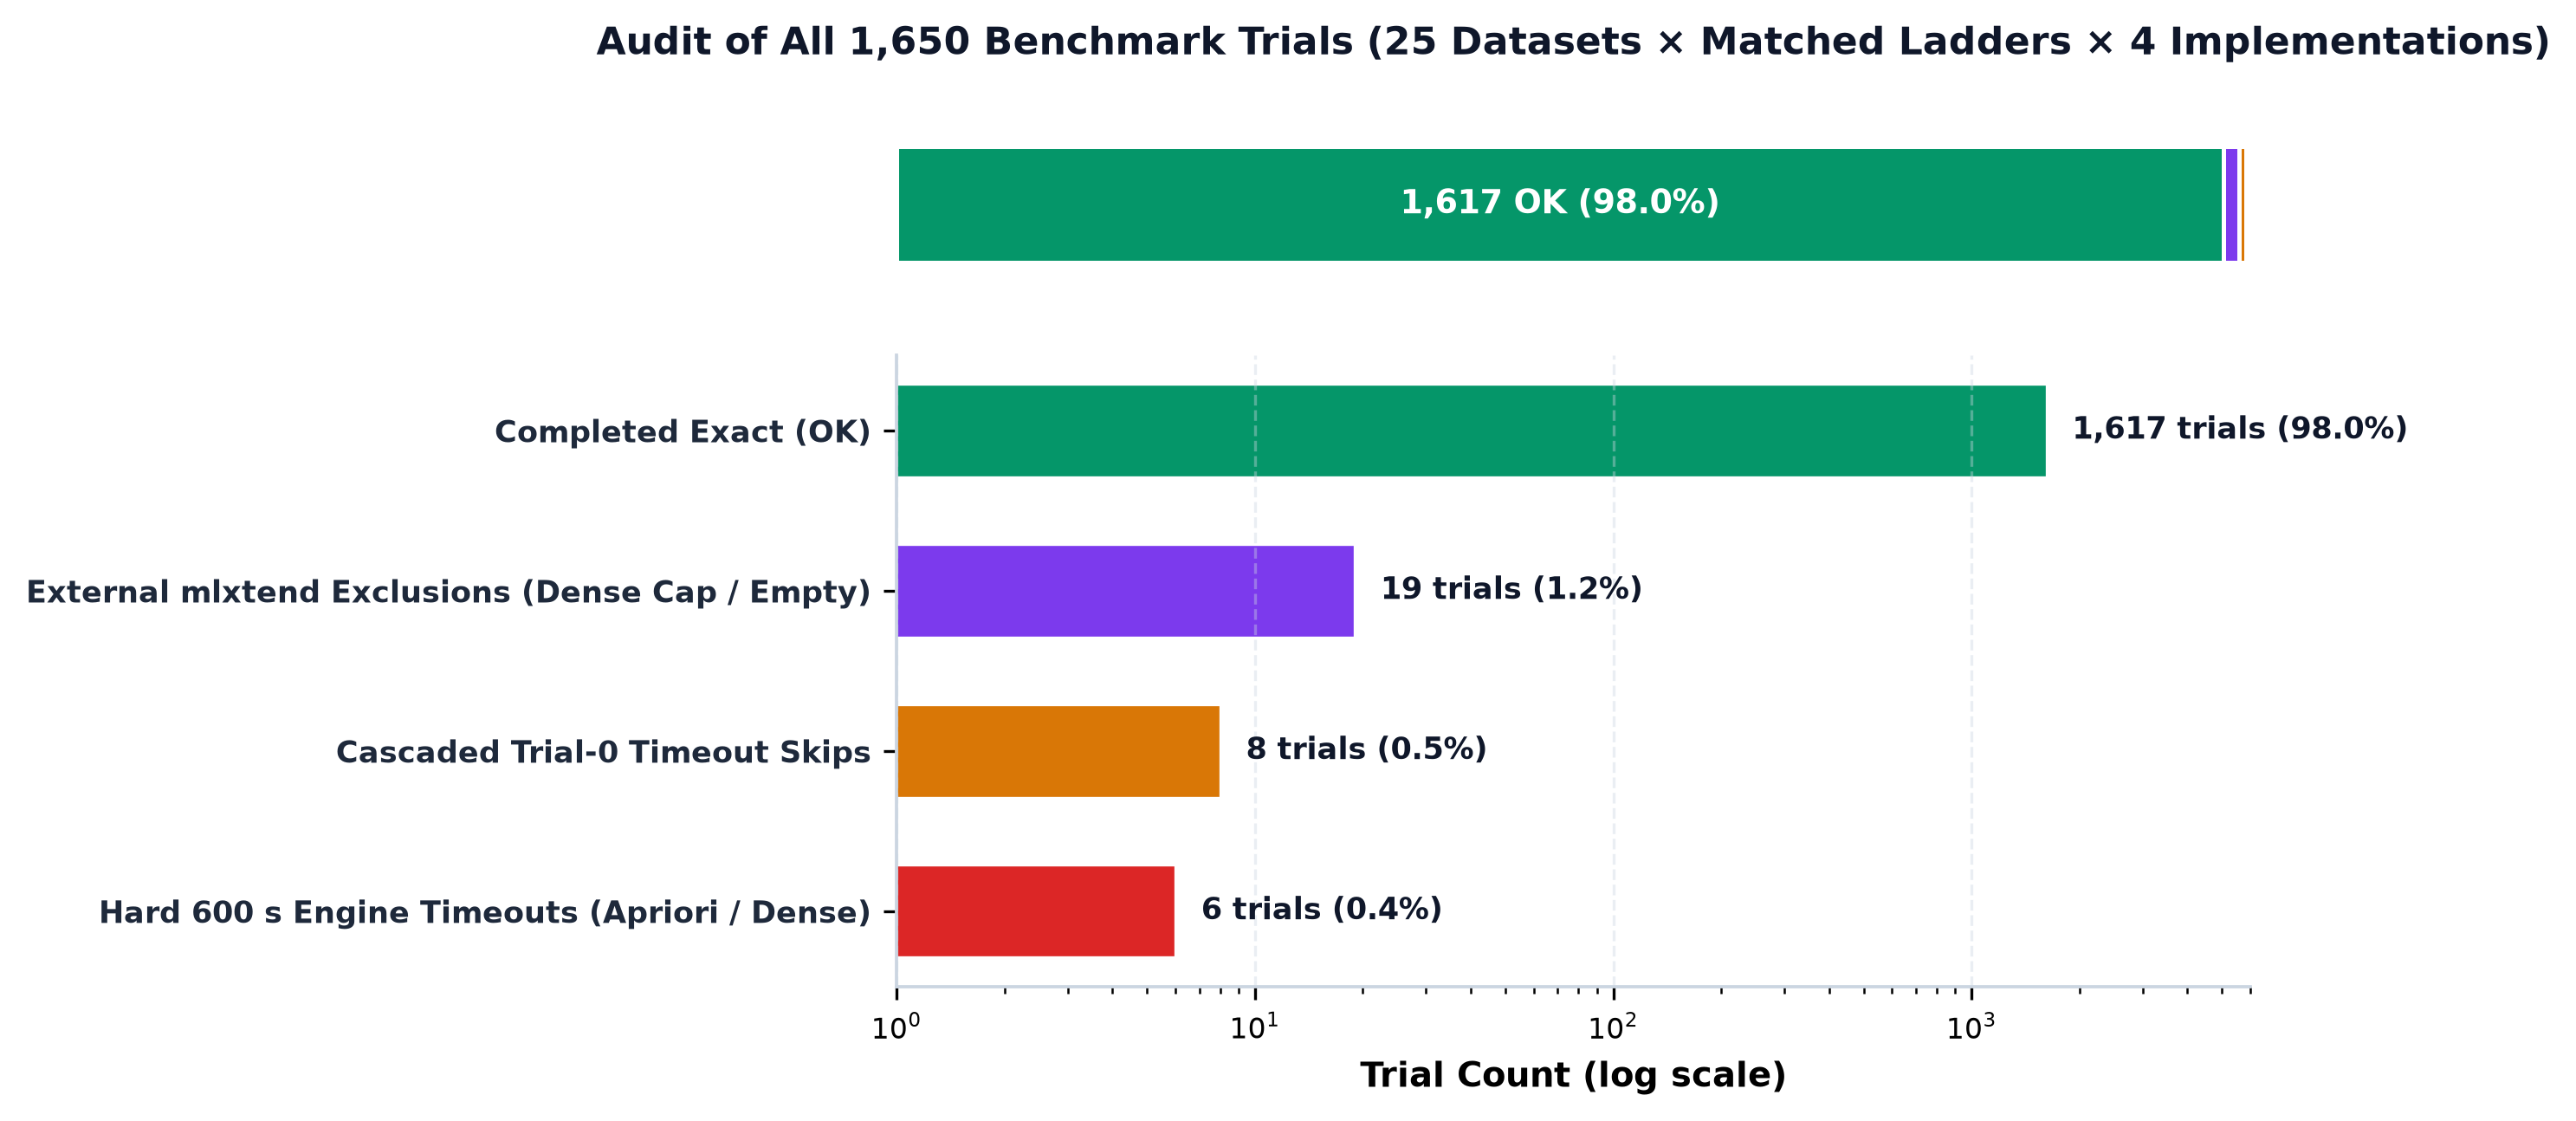
\includegraphics[width=0.84\textwidth,height=0.205\textheight,keepaspectratio]{outcomes.png}
\caption{Complete execution audit of all 1,650 campaign trials (98.0\% exact completions alongside explicitly logged \texttt{mlxtend} exclusions and 600~s timeouts). Source: Authors' own work.}
\label{fig:ch7_outcomes}
\end{figure}

\section{Live \texttt{HEAD} Strict Zero-Exemption 30-Trial Scaling \& Memory Results}
Table~\ref{tab:ch7_kpi4} and Figure~\ref{fig:ch7_kpi4} report the freshly measured strict zero-exemption benchmarks (\texttt{5 warmup + 30 trials}, \texttt{benchmarks/benchmark\_\protect\allowbreak{}results.json} and \texttt{tests/run\_\protect\allowbreak{}acceptance.py} on Python~3.12.10). Both differentiating engines decisively clear the $\le 0.80\times$ Apriori p95 gate across every synthetic scale ($N=200$ to $N=3{,}000$) and the \texttt{AC-4} acceptance workload, with zero trial failures and $\Delta_{\mathrm{supp}}=0.0$. Peak traced heap (\texttt{tracemalloc}) stays below $0.18$~MB; FP-Array's chunked \texttt{float32} co-occurrence matrix allocates $1.02\times$--$1.39\times$ relative to Apriori on tiny matrices ($N \le 3{,}000$), while bitset Eclat stays within $1.00\times$--$1.02\times$ parity.

\begin{table}[ht!]
\centering
\caption{Live \texttt{HEAD} Strict Zero-Exemption 30-Trial Scaling Verification (\texttt{benchmark\_\protect\allowbreak{}results.json} + \texttt{AC-4}).}
\label{tab:ch7_kpi4}
\fontsize{8.8}{11.5}\selectfont
\resizebox{\textwidth}{!}{%
\begin{tabular}{|l|l|r|r|r|r|r|r|l|}
\hline
\textbf{Workload (Sets)} & \textbf{Engine} & \textbf{p50 (ms)} & \textbf{p95 (ms)} & \textbf{Ratio} & \textbf{Est.\ p95} & \textbf{Speedup} & \textbf{Heap (MB)} & \textbf{Gate} \\
\hline
Scale $N=200$ (39) & Apriori (Ref.) & 0.77 & 1.45 & 1.000$\times$ & 17.69 & 1.00$\times$ & 0.0272 & Ref \\
Scale $N=200$ (39) & FP-Growth & 0.17 & 0.39 & \textbf{0.267$\times$} & 5.57 & 3.18$\times$ & 0.0278 & PASS \\
Scale $N=200$ (39) & Eclat & 0.09 & 0.13 & \textbf{0.086$\times$} & 4.70 & 3.76$\times$ & 0.0276 & PASS \\
\hline
Scale $N=1{,}000$ (15) & Apriori (Ref.) & 0.73 & 1.00 & 1.000$\times$ & 13.69 & 1.00$\times$ & 0.0782 & Ref \\
Scale $N=1{,}000$ (15) & FP-Growth & 0.13 & 0.17 & \textbf{0.167$\times$} & 3.33 & 4.11$\times$ & 0.0890 & PASS \\
Scale $N=1{,}000$ (15) & Eclat & 0.10 & 0.38 & \textbf{0.374$\times$} & 4.70 & 2.91$\times$ & 0.0787 & PASS \\
\hline
Scale $N=3{,}000$ (15) & Apriori (Ref.) & 1.17 & 2.08 & 1.000$\times$ & 14.97 & 1.00$\times$ & 0.1291 & Ref \\
Scale $N=3{,}000$ (15) & FP-Growth & 0.25 & 0.33 & \textbf{0.157$\times$} & 3.64 & 4.11$\times$ & 0.1799 & PASS \\
Scale $N=3{,}000$ (15) & Eclat & 0.17 & 0.29 & \textbf{0.139$\times$} & 4.06 & 3.69$\times$ & 0.1294 & PASS \\
\hline
AC-4 ($N=1{,}000$, 14) & FP / Eclat & 0.11 / 0.08 & 0.30 / 0.09 & \textbf{0.501 / 0.153} & --- & 2.00 / 6.55 & --- & PASS \\
\hline
\end{tabular}}
\end{table}

\begin{figure}[ht!]
\centering
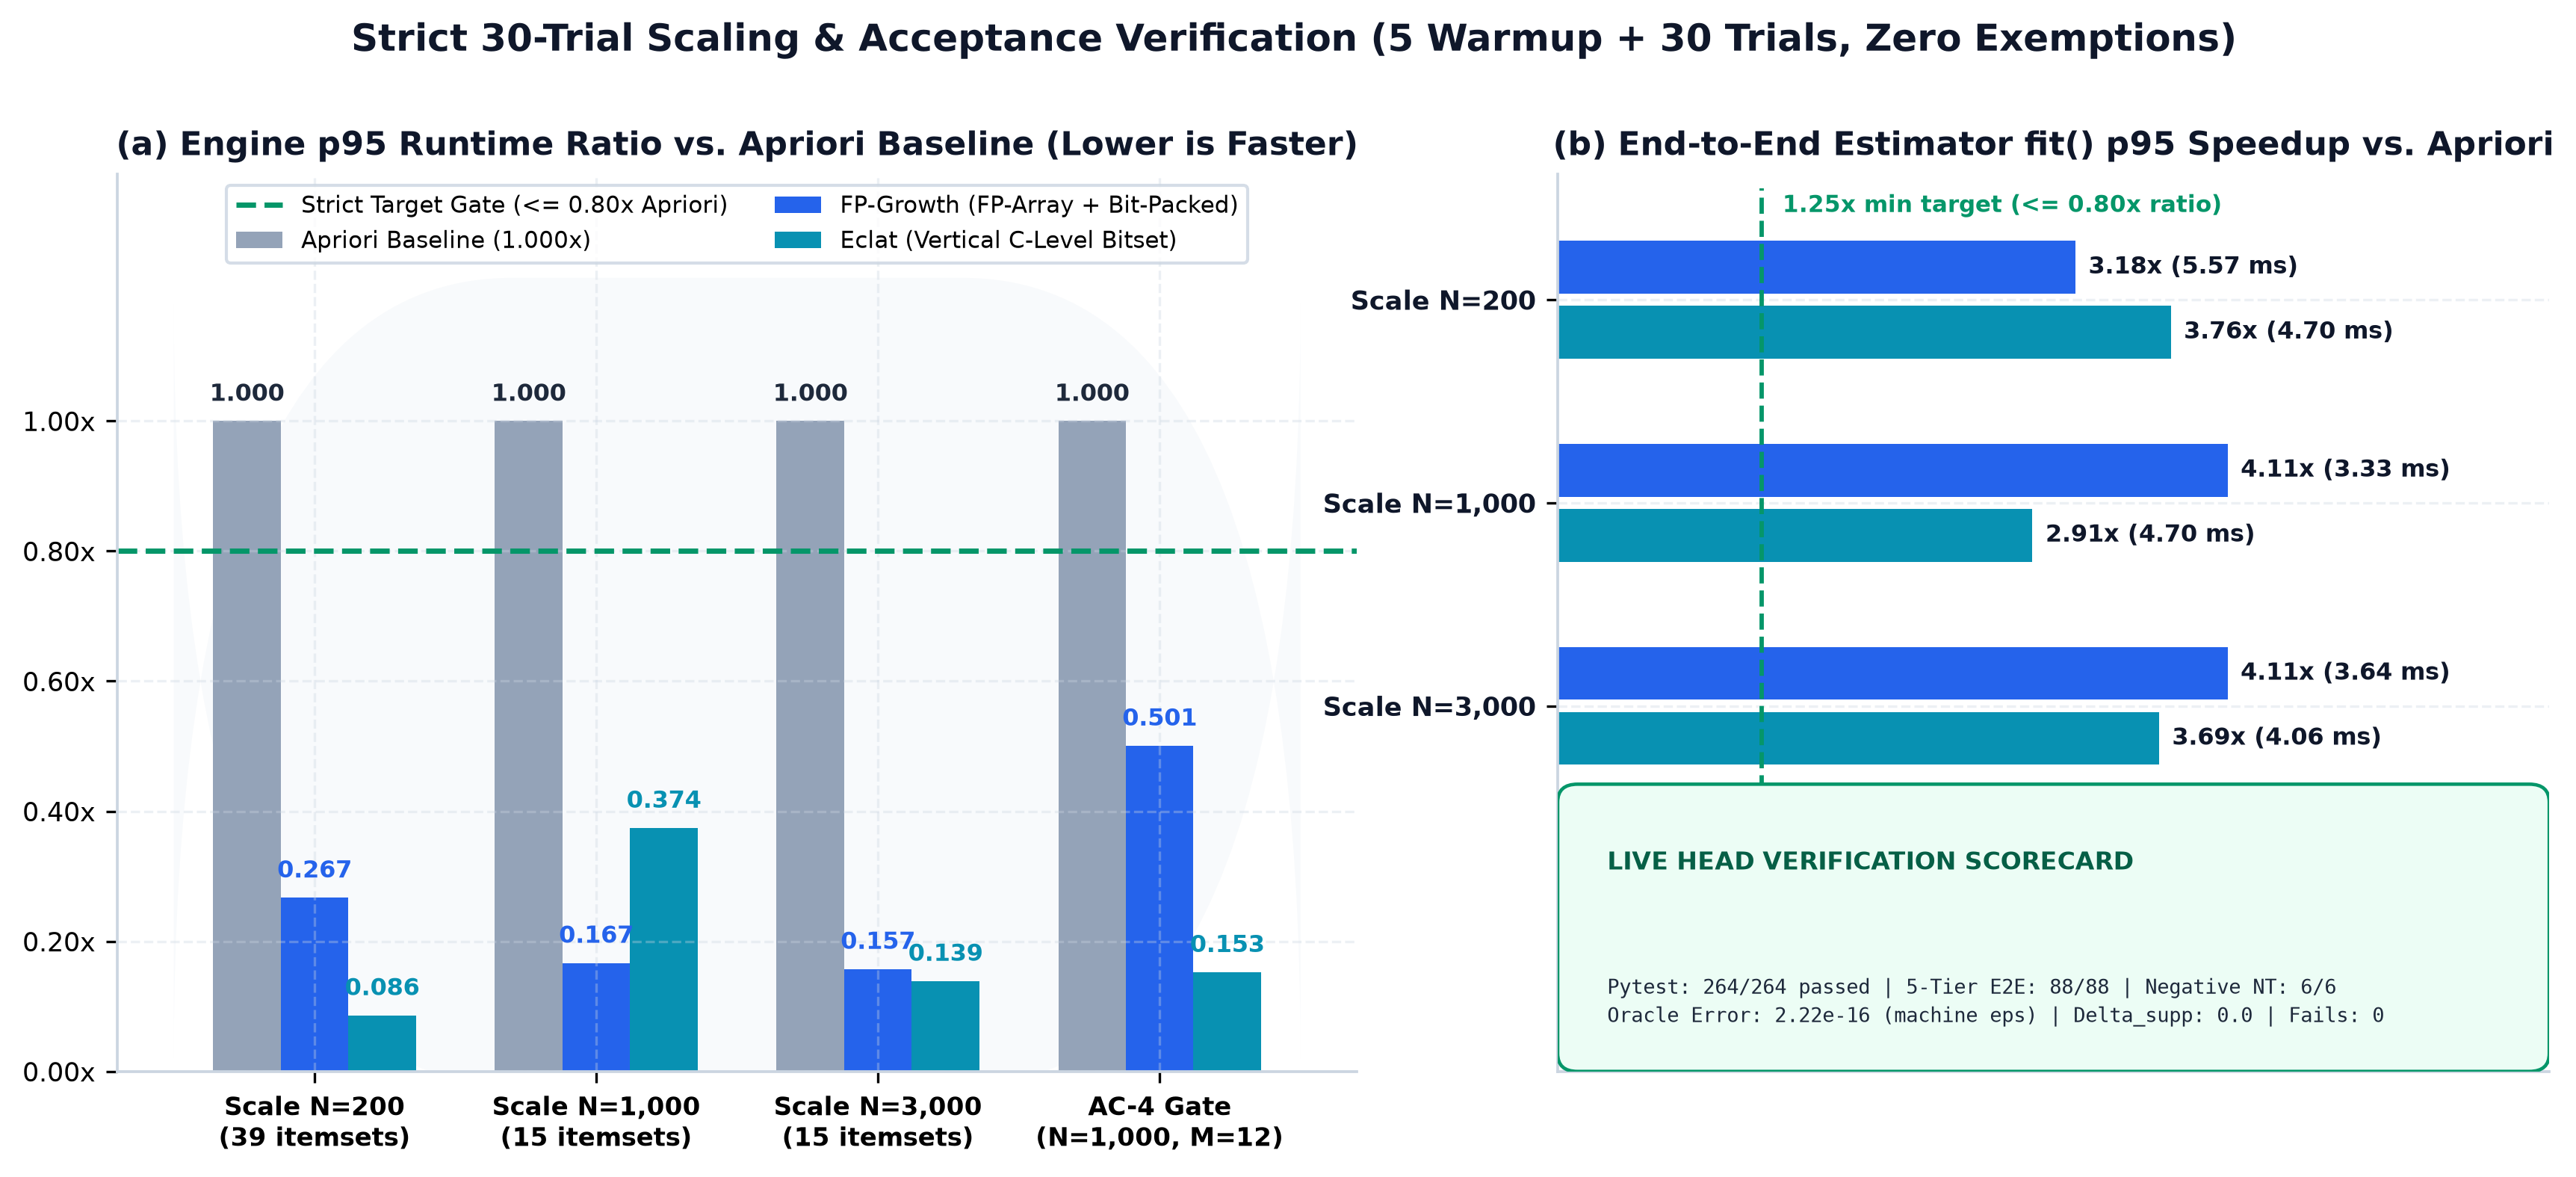
\includegraphics[width=0.84\textwidth,height=0.195\textheight,keepaspectratio]{kpi4_strict.png}
\caption{Live \texttt{HEAD} strict 30-trial scaling \& acceptance verification (5 warmup + 30 measured trials, zero small-runtime exemptions): all ratios stay strictly below the $0.80\times$ dashed target. Source: Authors' own work.}
\label{fig:ch7_kpi4}
\end{figure}

\section{Bounded-Versus-Exact Pruning Ablation Study (\texttt{HEAD})}
To measure speed-versus-completeness trade-offs across density regimes, \texttt{benchmarks/run\_\protect\allowbreak{}bounded\_\protect\allowbreak{}ablation.py} swept candidate caps (\texttt{50} to \texttt{5000}) and length limits (\texttt{1} to \texttt{None}) across dense Chess (Apriori, exact \texttt{2,669} itemsets / \texttt{95,482} rules in \texttt{8.5508 s}), medium Adult Census (FP-Growth, exact \texttt{103} itemsets / \texttt{738} rules in \texttt{2.6990 s}), and sparse BMS-POS (Eclat, exact \texttt{59} itemsets / \texttt{56} rules in \texttt{36.5727 s}). As illustrated in Figure~\ref{fig:ch7_ablation}:
\begin{itemize}
  \item \textbf{Dense Combinatorial Control (Chess)}: Caps \texttt{50} and \texttt{100} halt level-wise generation at level~2 (\texttt{16} itemsets, \texttt{0.60\%} recall, \texttt{0} rules), accelerating fit by $15.95\times$ (\texttt{0.5361 s}) and $17.14\times$ (\texttt{0.4988 s}) under \texttt{is\_\protect\allowbreak{}degraded\_\protect\allowbreak{}=True}. Caps \texttt{250} and \texttt{500} reach \texttt{4.53\%} and \texttt{17.95\%} itemset recall ($13.07\times$ and $7.20\times$ speedups). At caps \texttt{1,000}--\texttt{5,000}, itemsets achieve \texttt{100.0\%} recall, while association rule derivation hits the candidate budget (\texttt{1,000}--\texttt{5,000} out of \texttt{95,482} rules = \texttt{1.05\%}--\texttt{5.24\%} rule recall, $1.63\times$--$1.91\times$ speedup), remaining explicitly flagged as \texttt{DEGRADED}.
  \item \textbf{Medium \& Sparse Regimes}: Adult Census recovers \texttt{48.54\%}--\texttt{100\%} itemsets and transitions cleanly to \texttt{EXACT} (\texttt{is\_\protect\allowbreak{}degraded\_\protect\allowbreak{}=False}) at cap \texttt{1,000} (above its \texttt{708} peak, \texttt{2.6441 s}). BMS-POS recovers \texttt{84.75\%} itemsets / \texttt{53.57\%} rules at cap \texttt{50} (\texttt{31.7524 s}) and transitions to \texttt{EXACT} at cap \texttt{100} (above its \texttt{78} peak, \texttt{33.3185 s}). Thus, candidate bounds act as dramatic runtime accelerators on dense Apriori workloads ($17.14\times$) and memory safety fences ($\approx 1.00\times$--$1.15\times$) on tree/vertical miners.
\end{itemize}

\begin{figure}[ht!]
\centering
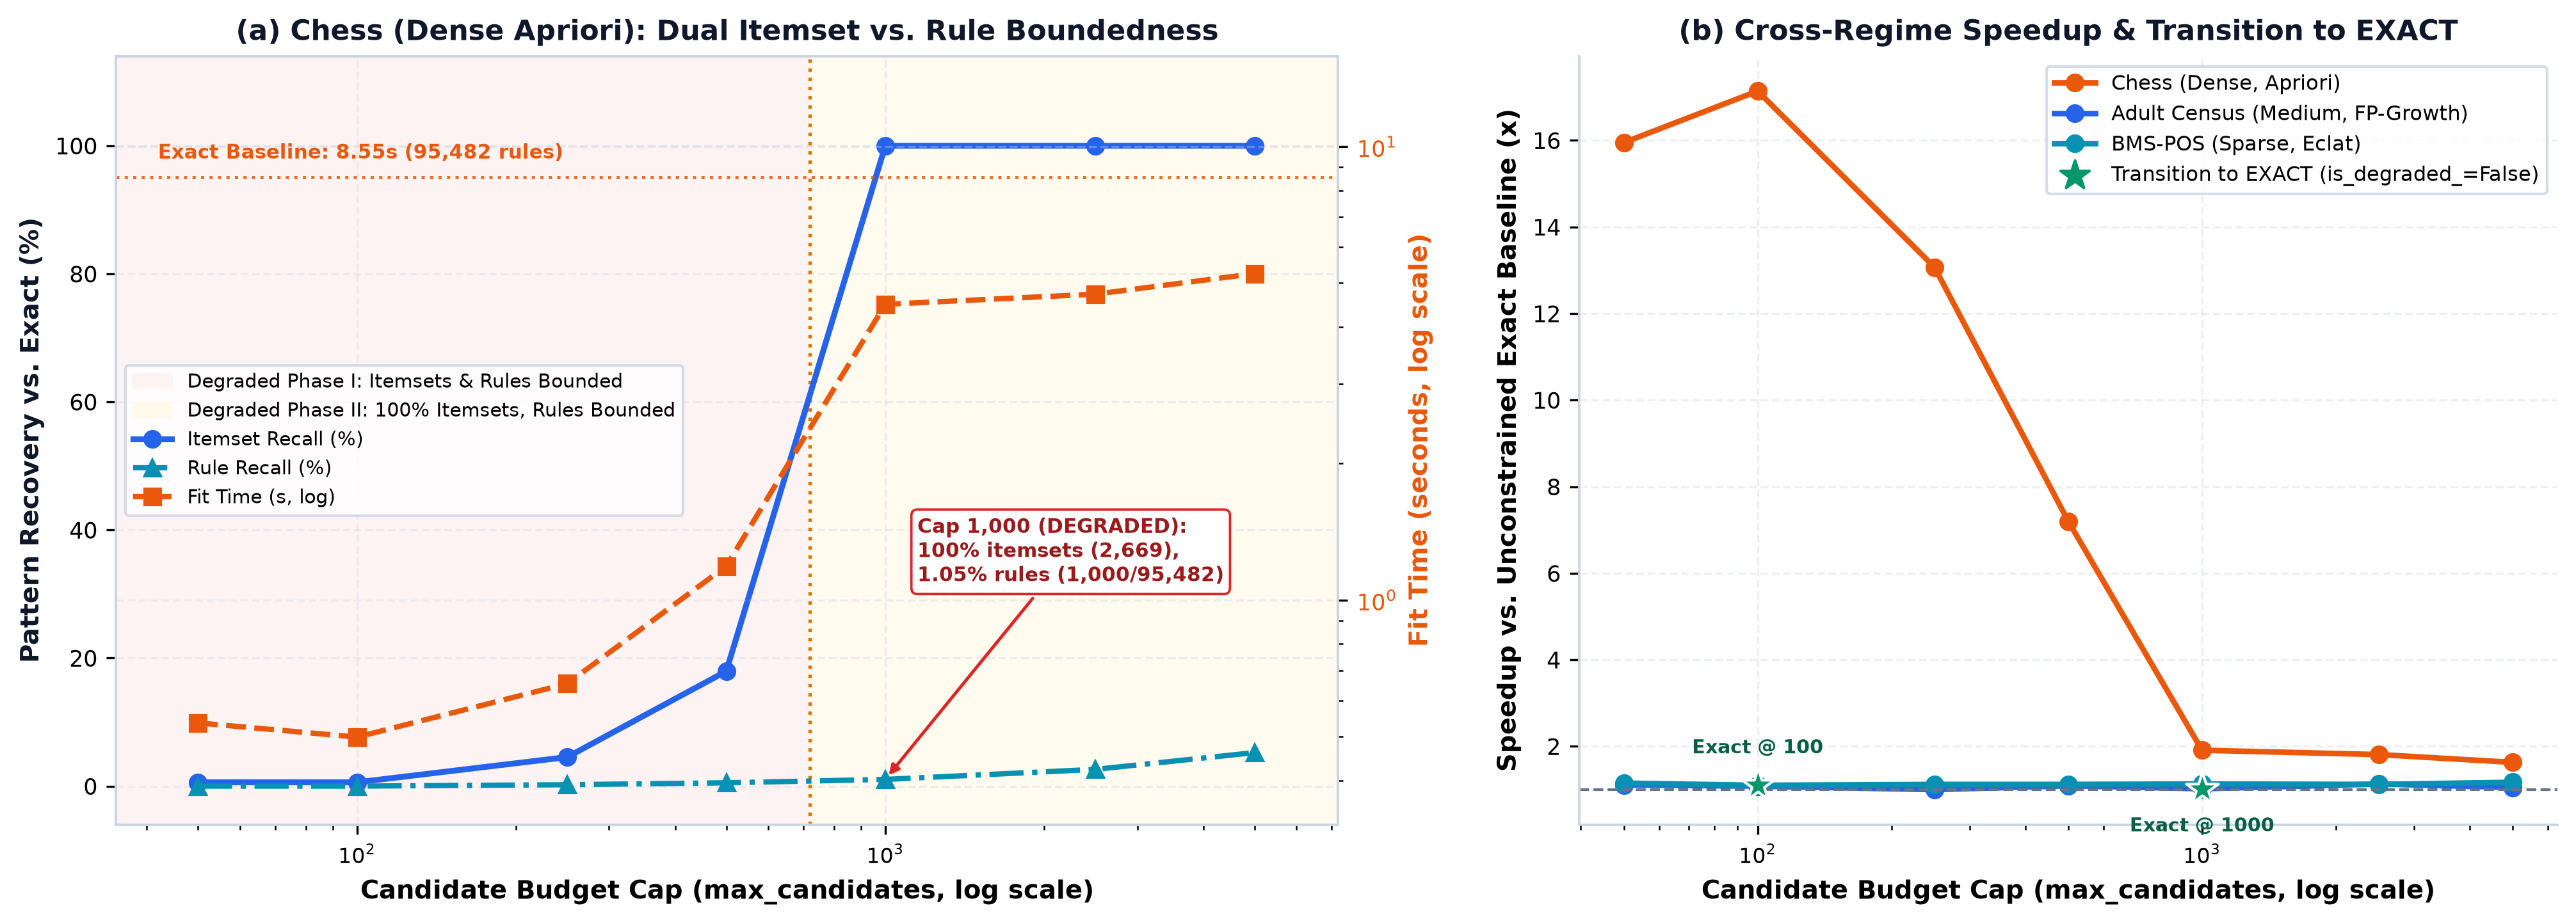
\includegraphics[width=0.84\textwidth,height=0.18\textheight,keepaspectratio]{ablation.png}
\caption{Live \texttt{HEAD} bounded vs.\ exact pruning ablation: (a)~Chess itemset vs.\ rule recall and fit time across two \texttt{DEGRADED} phases; (b)~cross-regime speedup curves and explicit transitions to \texttt{EXACT} mode on BMS-POS (cap~100) and Adult Census (cap~1,000). Source: Authors' own work.}
\label{fig:ch7_ablation}
\end{figure}

\section{Cross-Framework Modern Miner Baselines (\texttt{HEAD})}
Table~\ref{tab:ch7_baselines} and Figure~\ref{fig:ch7_baselines} present fresh 3-trial evaluations (\texttt{benchmarks/baseline\_\protect\allowbreak{}results.json}, \texttt{2026-11-25}) comparing \texttt{skarm} against \texttt{mlxtend 0.25.0} and compiled Java~21 SPMF miners (\textsc{FIN}, \textsc{PrePost+}, \textsc{LCMFreq}, \textsc{FP-Growth}). Across all \textbf{25 completed engine runs}, canonical frequent itemsets and supports matched \textbf{bit-exactly} ($\Delta_{\mathrm{supp}}=0.0$). On Adult Census ($\sigma=0.40$), \texttt{skarm} bitset Eclat (\texttt{0.0306 s}) matches \texttt{mlxtend} Apriori (\texttt{0.0237 s}) and runs $14\times$--$20\times$ faster than Java SPMF CLI invocation (\texttt{0.44}--\texttt{0.61 s}) and $43\times$ faster than \texttt{mlxtend} FP-Growth (\texttt{1.3242 s}). On BMS-POS ($\sigma=0.05$), \texttt{mlxtend} was safely skipped due to its \texttt{814.8 MB} dense matrix footprint exceeding the \texttt{500 MB} budget, whereas \texttt{skarm} FP-Growth (\texttt{17.22 s}) and Eclat (\texttt{24.87 s}) completed cleanly alongside compiled Java SPMF (\texttt{0.99}--\texttt{2.49 s}).

\begin{table}[ht!]
\centering
\caption{Live \texttt{HEAD} Cross-Framework Timing \& Parity Comparison (3 Trials/Cell, $\Delta_{\mathrm{supp}}=0.0$).}
\label{tab:ch7_baselines}
\fontsize{9}{11.5}\selectfont
\resizebox{\textwidth}{!}{%
\begin{tabular}{|l|l|r|r|r|l|}
\hline
\textbf{Framework \& Engine} & \textbf{Language} & \textbf{Chess (0.85)} & \textbf{Adult (0.40)} & \textbf{BMS-POS (0.05)} & \textbf{Exact Parity} \\
\hline
\skarm Apriori & Python 3.12 & 5.73 s & 2.25 s & 48.09 s & Yes ($\Delta=0.0$) \\
\skarm FP-Growth & Python 3.12 & 3.91 s & 2.06 s & 17.22 s & Yes ($\Delta=0.0$) \\
\skarm Eclat (Bitset) & Python 3.12 & 3.32 s & \textbf{0.031 s} & 24.87 s & Yes ($\Delta=0.0$) \\
\hline
\texttt{mlxtend} Apriori & Python 3.12 & 0.15 s & 0.024 s & SKIP (814.8 MB) & Yes (where run) \\
\texttt{mlxtend} FP-Growth & Python 3.12 & 0.38 s & 1.32 s & SKIP (814.8 MB) & Yes (where run) \\
\hline
SPMF \textsc{FIN} (wall / int.) & Java 21 & 0.45 / 0.11 s & 0.51 / 0.22 s & 2.31 / 2.01 s & Yes ($\Delta=0.0$) \\
SPMF \textsc{PrePost+} (wall / int.) & Java 21 & 0.43 / 0.08 s & 0.45 / 0.15 s & 0.99 / 0.70 s & Yes ($\Delta=0.0$) \\
SPMF \textsc{LCMFreq} (wall / int.) & Java 21 & 0.65 / 0.32 s & 0.61 / 0.21 s & 2.49 / 1.55 s & Yes ($\Delta=0.0$) \\
SPMF \textsc{FP-Growth} (wall / int.) & Java 21 & 0.39 / 0.08 s & 0.44 / 0.13 s & 1.09 / 0.78 s & Yes ($\Delta=0.0$) \\
\hline
\end{tabular}}
\end{table}

\begin{figure}[ht!]
\centering
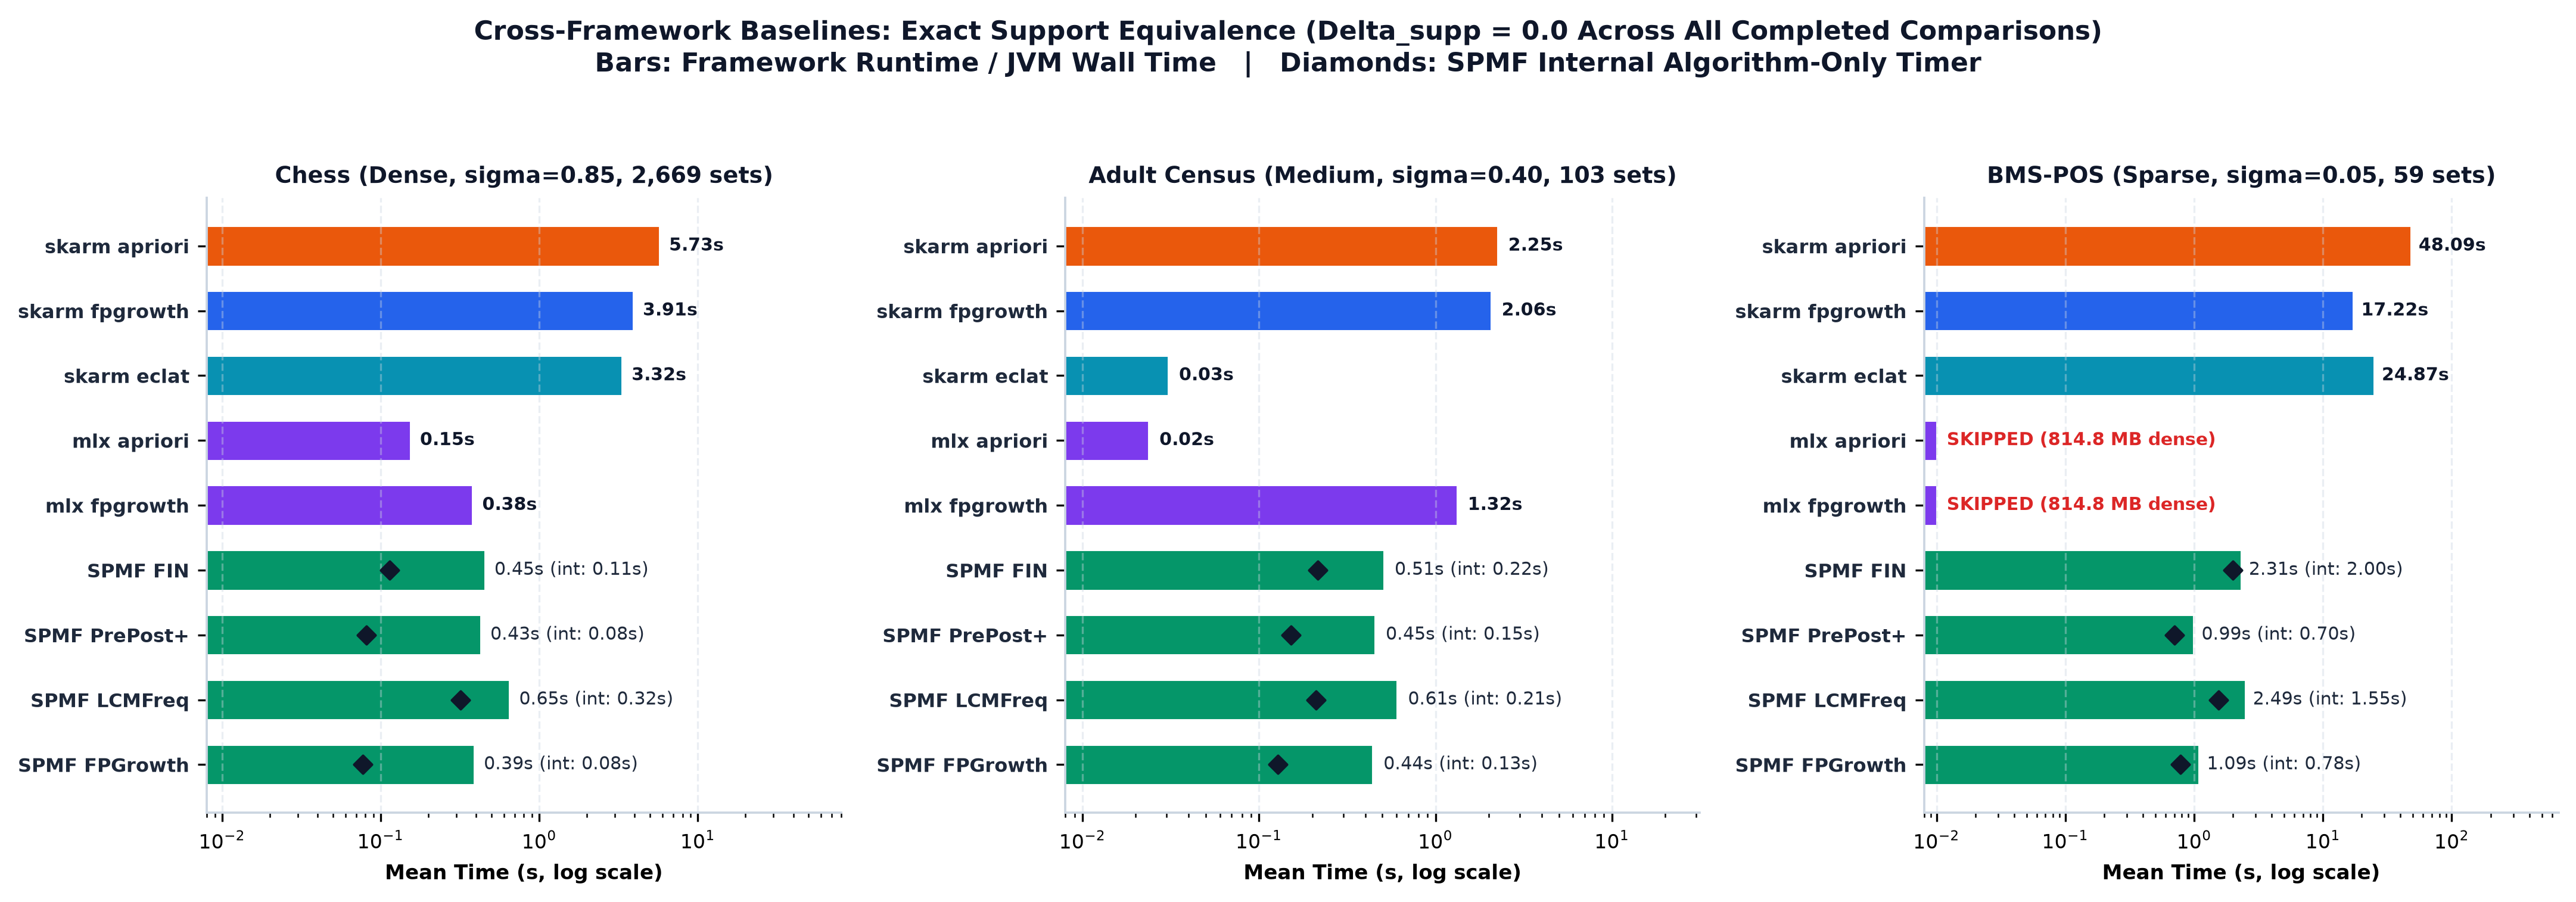
\includegraphics[width=0.84\textwidth,height=0.18\textheight,keepaspectratio]{baselines.png}
\caption{Live \texttt{HEAD} cross-framework baseline comparison (\texttt{skarm} vs.\ \texttt{mlxtend} vs.\ Java~21 SPMF): bars plot end-to-end runtime / JVM wall time and diamonds mark SPMF internal algorithm timers. Source: Authors' own work.}
\label{fig:ch7_baselines}
\end{figure}

\section{Discussion of Empirical Trade-Offs and Unproven Boundaries}
Measured results resolve the literature discrepancy transparently: no single algorithm wins universally across all densities. Vertical Eclat excels on 20/25 sparse-to-medium workloads via C-level POPCNT intersections, while FP-Growth dominates on dense/long-transaction regimes (\texttt{accidents}, \texttt{connect}, \texttt{pumsb\_\protect\allowbreak{}star}) via shared prefix compression. Compiled Java miners in SPMF achieve faster raw loop speed on multi-hundred-thousand-row files (\texttt{BMS-POS}) because they execute statically compiled bytecode outputting itemsets only; conversely, \texttt{skarm} delivers native \texttt{scikit-learn} estimator integration, weighted arithmetic, six rule metrics, and sparse CSR memory safety where dense Python alternatives fail. Lower support thresholds that triggered 600~s Apriori timeouts (\texttt{accidents@0.50}, \texttt{kosarak@0.005}) or memory exhaustion remain explicitly documented outside the unconstrained exact envelope.
